\documentclass[oneside]{VUMIFPSkursinis}
\usepackage{algorithmicx}
\usepackage{algorithm}
\usepackage{algpseudocode}
\usepackage{amsfonts}
\usepackage{float}
\usepackage{amsmath}
\usepackage{bm}
\usepackage{caption}
\usepackage{color}
\usepackage{float}
\usepackage{graphicx}
\usepackage{listings}
\usepackage{subfig}
\usepackage{ltablex}
\usepackage{longtable}
\usepackage{wrapfig}
\usepackage{subfig}
\usepackage{pbox}
\renewcommand{\labelenumii}{\theenumii}
\renewcommand{\theenumii}{\theenumi.\arabic{enumii}.}
\renewcommand{\labelenumiii}{\theenumiii}
\renewcommand{\theenumiii}{\theenumii\arabic{enumiii}.}
\newcolumntype{P}[1]{>{\centering\arraybackslash}p{#1}}
\usepackage[%  
    colorlinks=true,
    linkcolor=black
]{hyperref}
\university{Vilniaus universitetas}
\faculty{Matematikos ir informatikos fakultetas}
\department{Programų sistemų katedra}
\papertype{Programų sistemų inžinerija II laboratorinis darbas II}
\title{Reikalavimų analizė ir techninė architektūra}
\titleineng{Requirements Analysis and Technical Architecture}
\status{2 kurso 3 grupės studentai}



\supervisor{Audronė Lupeikienė, M. Darbuot., Dr.}
\date{Vilnius – \the\year}

\bibliography{bibliografija}

\begin{document}
\maketitle
\tableofcontents

\section{Anotacija}
\begin{itemize}
	\item{Matas Savickis}
	\item{Justas Tvarijonas}
	\item{Rytautas Kvasinskas}
	\item{Greta Pyrantaitė}
	\item{Tomas Kiziela}
\end{itemize}

\section{Sistemos detalus projektas}
	\subsection{Sistemos užduotys}
		\subsubsection{Užduočių diagramos}


			\begin{figure}[h]
    				\centering
    				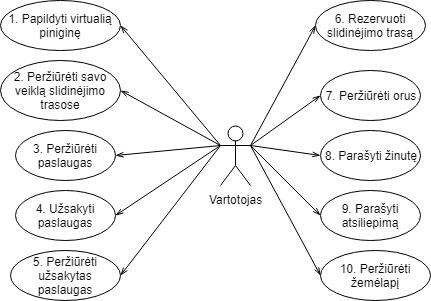
\includegraphics[width=0.75\textwidth]{useCaseVartotojas.png}
    				\caption{Vartotojo užduočių diagrama}
    				\label{fig:VartotojoUseCasel}
			\end{figure}
\pagebreak

	\subsubsection{Robastiškumo diagramos}

			\begin{figure}[h]
    				\centering
    				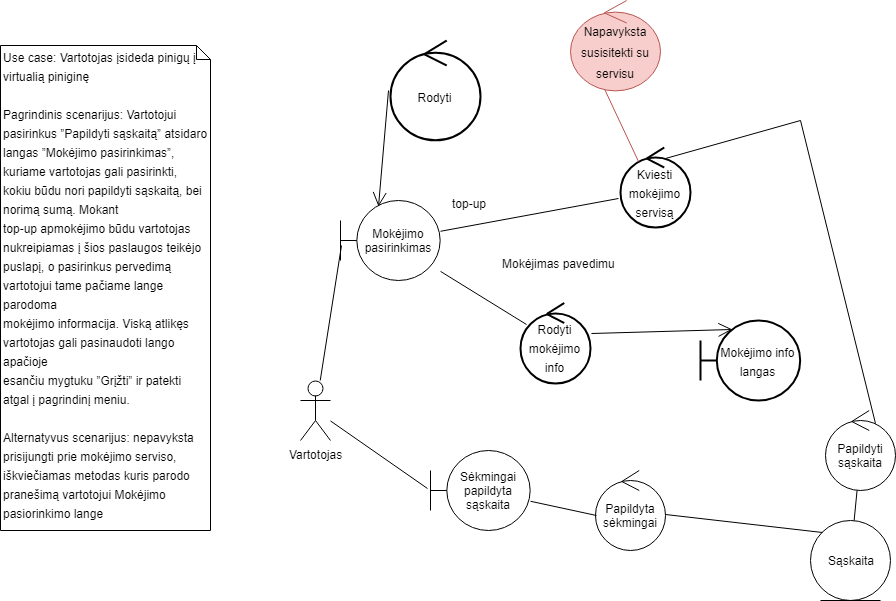
\includegraphics[width=1\textwidth]{rob1.png}
    				\caption{Vartotojas įsideda pinigų į virtualią piniginę}
    				\label{fig:Vartotojas įsideda pinigų į virtualią piniginę}
			\end{figure}

			\begin{figure}[h]
    				\centering
    				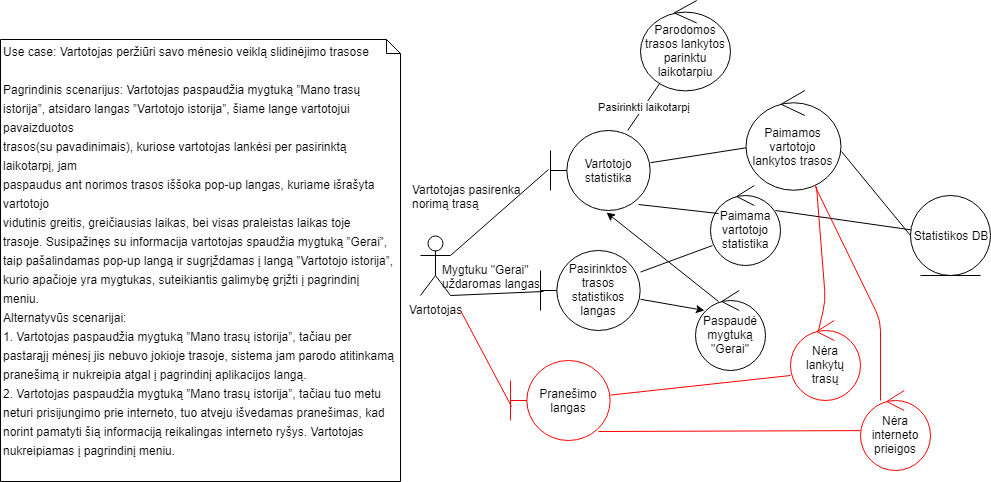
\includegraphics[width=1\textwidth]{rob2.png}
    				\caption{Vartotojas peržiūri savo veiklą trasose}
    				\label{fig:Vartotojas peržiūri savo veiklą trasose}
			\end{figure}

			\begin{figure}[h]
    				\centering
    				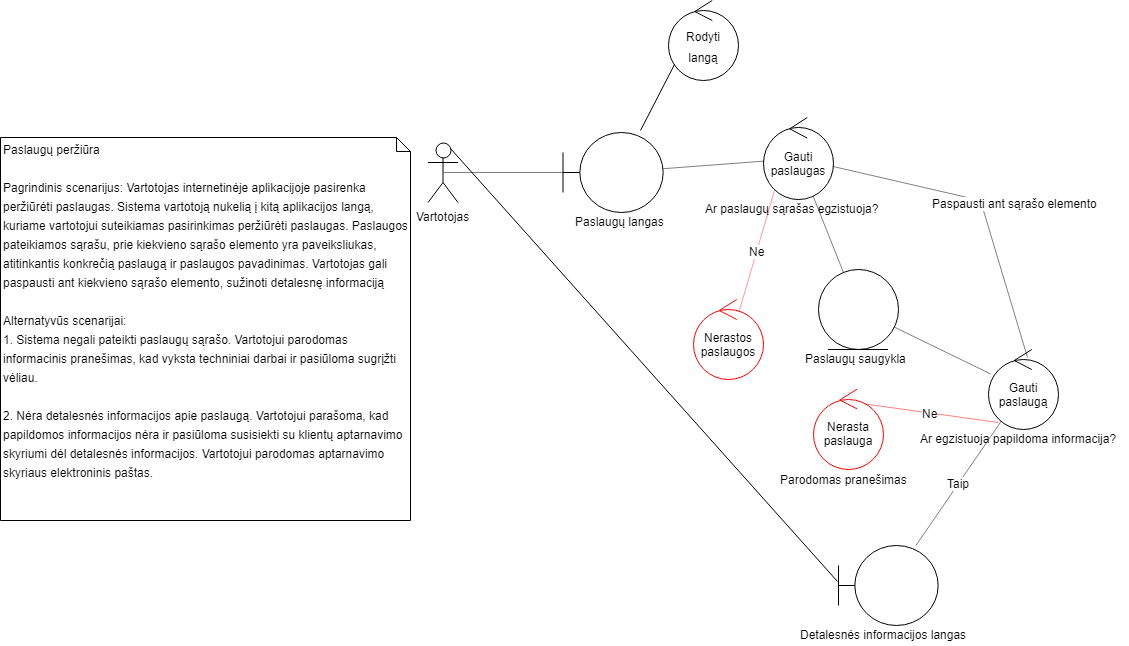
\includegraphics[width=1\textwidth]{rob4.png}
    				\caption{Paslaugų peržiūra}
    				\label{fig:Paslaugų peržiūra}
			\end{figure}

			\begin{figure}[h]
    				\centering
    				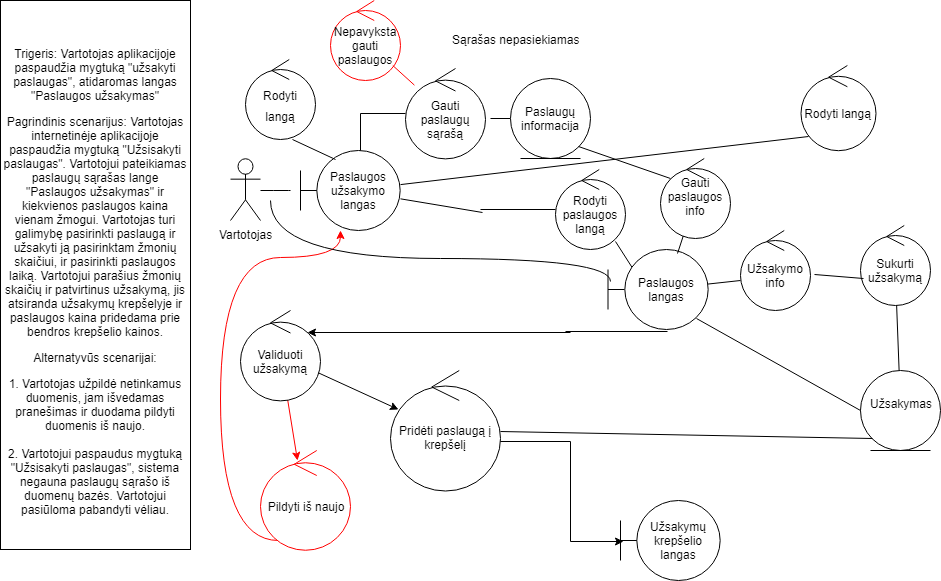
\includegraphics[width=1\textwidth]{rob6.png}
    				\caption{Vartotojas užsisako paslaugas}
    				\label{fig:Vartotojas užsisako paslaugas}
			\end{figure}

			\begin{figure}[h]
    				\centering
    				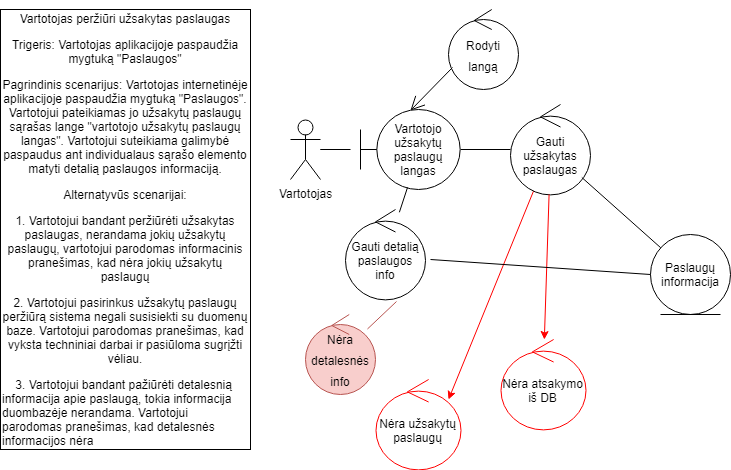
\includegraphics[width=1\textwidth]{rob7.png}
    				\caption{Vartotojas peržiūri užsakytas paslaugas}
    				\label{fig:Vartotojas peržiūri užsakytas paslaugas}
			\end{figure}

			\begin{figure}[h]
    				\centering
    				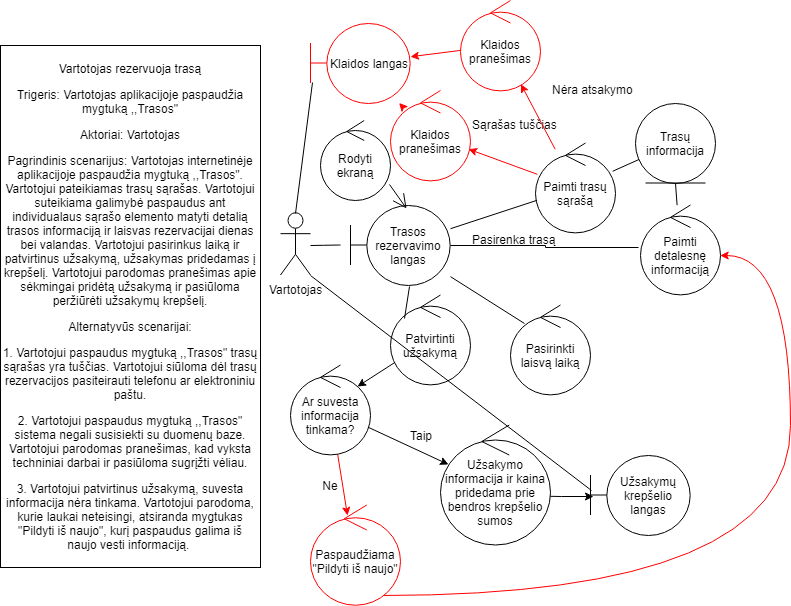
\includegraphics[width=1\textwidth]{rob8.png}
    				\caption{Vartotojas rezervuoja trasą}
    				\label{fig:VartotojoUseCasel}
			\end{figure}

			\begin{figure}[h]
    				\centering
    				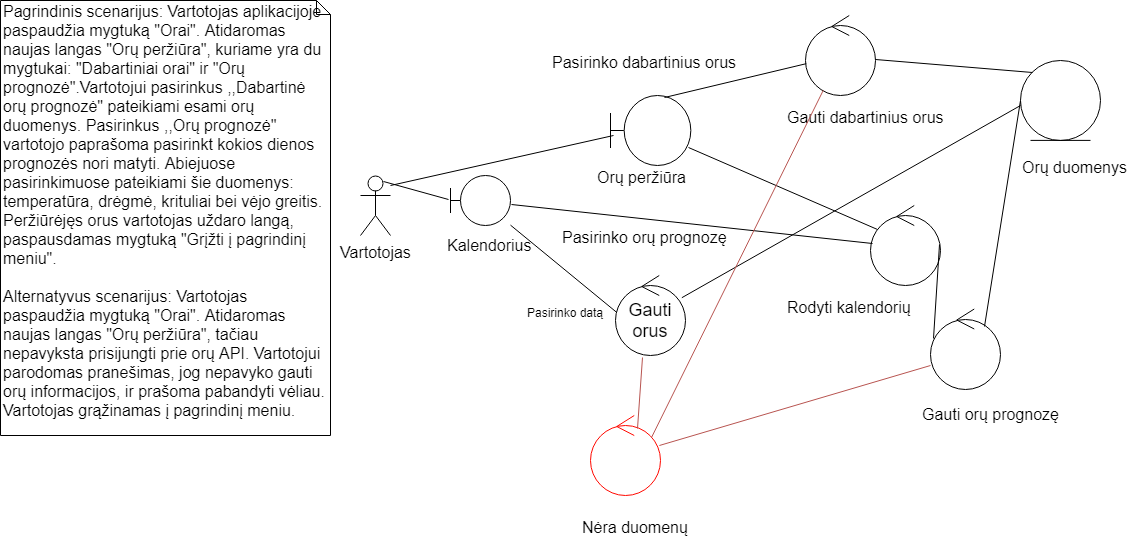
\includegraphics[width=1\textwidth]{rob10.png}
    				\caption{Vartotojas peržiūri orų prognozę}
    				\label{fig:Vartotojas peržiūri orų prognozę}
			\end{figure}

			\begin{figure}[h]
    				\centering
    				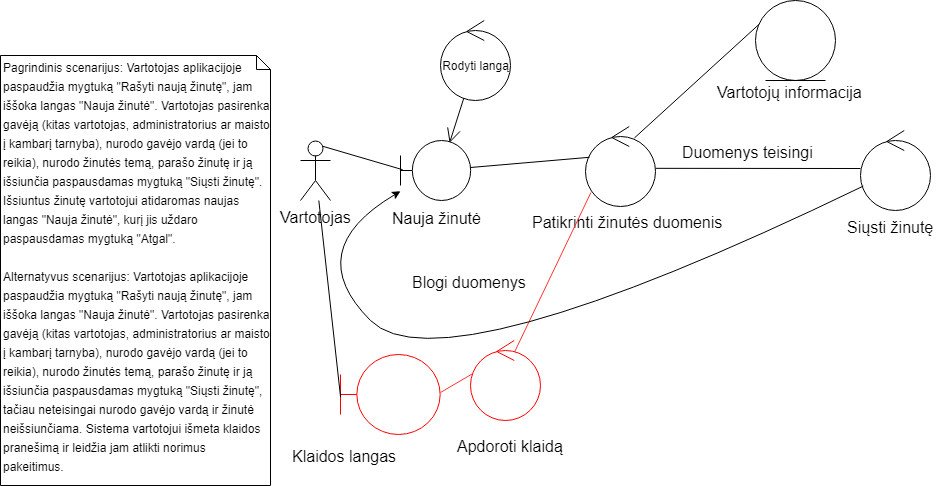
\includegraphics[width=1\textwidth]{rob11.png}
    				\caption{Vartotojas rašo žinutę}
    				\label{fig:Vartotojas rašo žinutę}
			\end{figure}

			\begin{figure}[h]
    				\centering
    				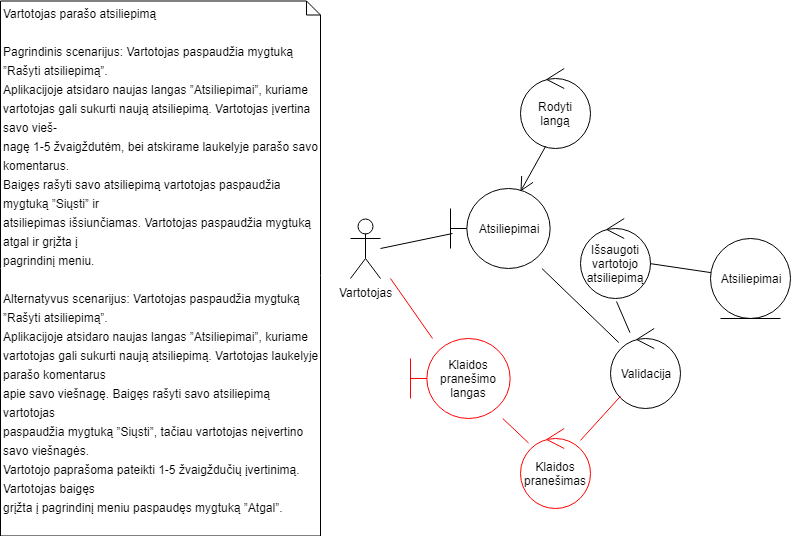
\includegraphics[width=1\textwidth]{rob12.png}
    				\caption{Vartotojas rašo atsiliepimą}
    				\label{fig:Vartotojas rašo atsiliepimą}
			\end{figure}

			\begin{figure}[h]
    				\centering
    				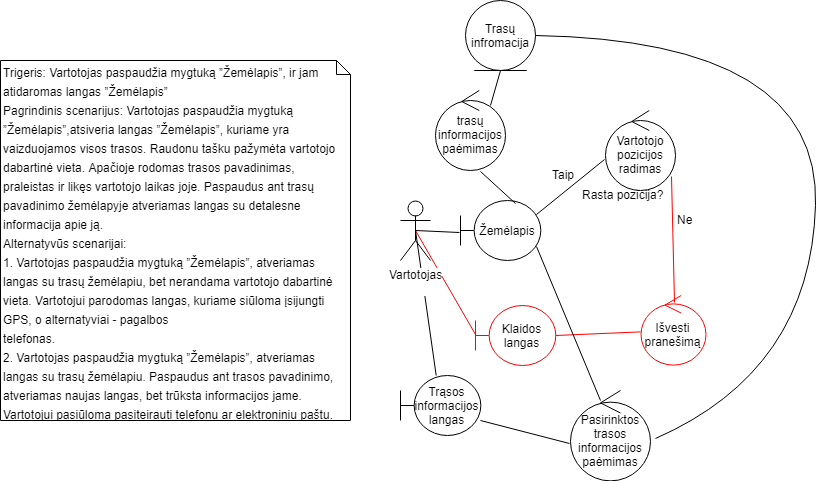
\includegraphics[width=1\textwidth]{rob13.png}
    				\caption{Vartotojas peržiūri žemėlapį}
    				\label{fig:Vartotojas peržiūri žemėlapį}
			\end{figure}

\section{Sekų diagramos}
			\begin{figure}[h]
    				\centering
    				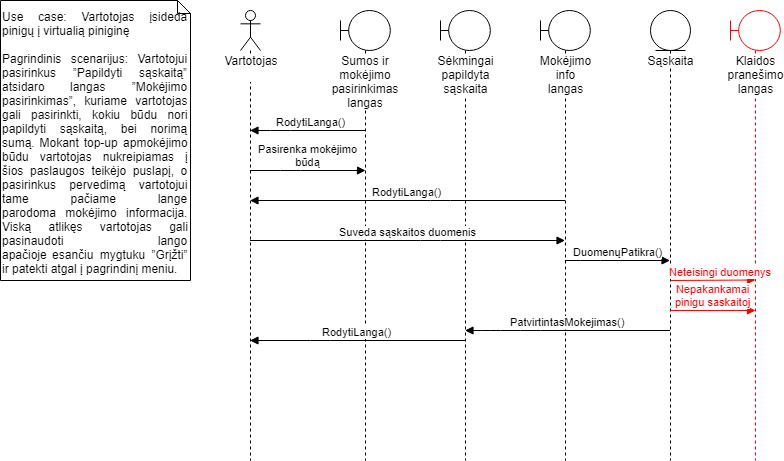
\includegraphics[width=1\textwidth]{seq1.png}
    				\caption{Vartotojas įsideda pinigų į virtualią piniginę}
    				\label{fig:Vartotojas įsideda pinigų į virtualią piniginę}
			\end{figure}

			\begin{figure}[h]
    				\centering
    				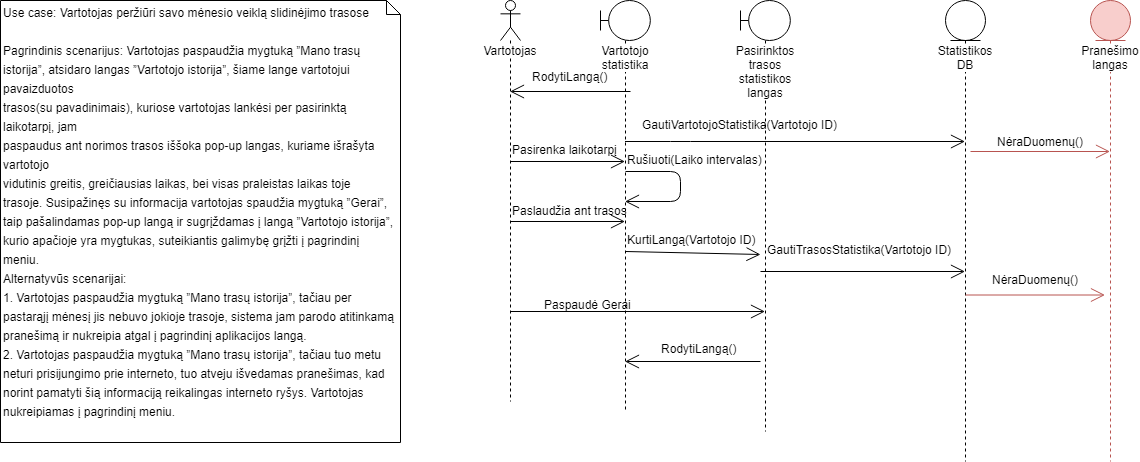
\includegraphics[width=1\textwidth]{seq2.png}
    				\caption{Vartotojas peržiūri savo veiklą trasose}
    				\label{fig:Vartotojas peržiūri savo veiklą trasose}
			\end{figure}


			\begin{figure}[h]
    				\centering
    				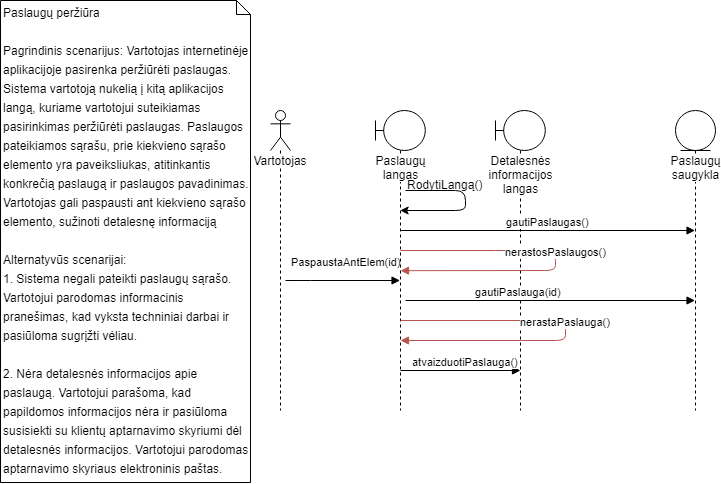
\includegraphics[width=1\textwidth]{seq4.png}
    				\caption{Paslaugų peržiūra}
    				\label{fig:Paslaugų peržiūra}
			\end{figure}

			\begin{figure}[h]
    				\centering
    				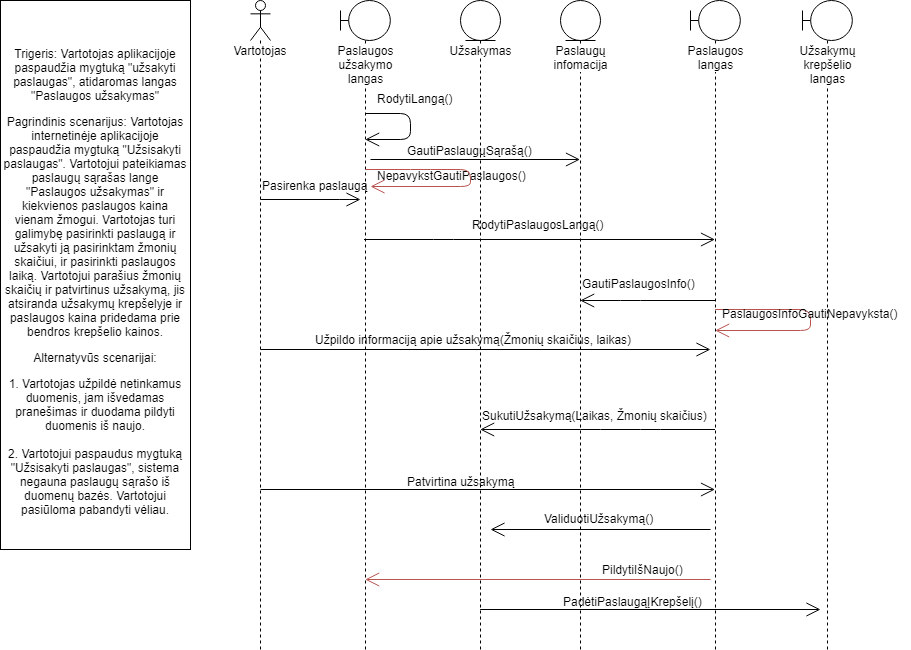
\includegraphics[width=1\textwidth]{seq6.png}
    				\caption{Vartotojas užsisako paslaugas}
    				\label{fig:Vartotojas užsisako paslaugas}
			\end{figure}

			\begin{figure}[h]
    				\centering
    				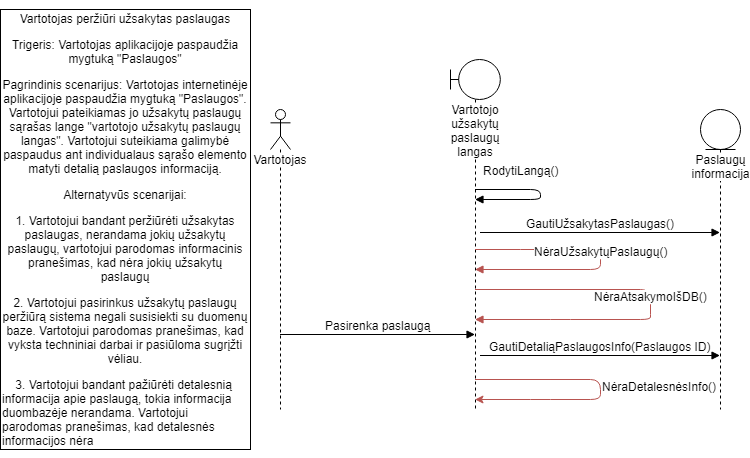
\includegraphics[width=1\textwidth]{seq7.png}
    				\caption{Vartotojas peržiūri užsakytas paslaugas}
    				\label{fig:Vartotojas peržiūri užsakytas paslaugas}
			\end{figure}

			\begin{figure}[h]
    				\centering
    				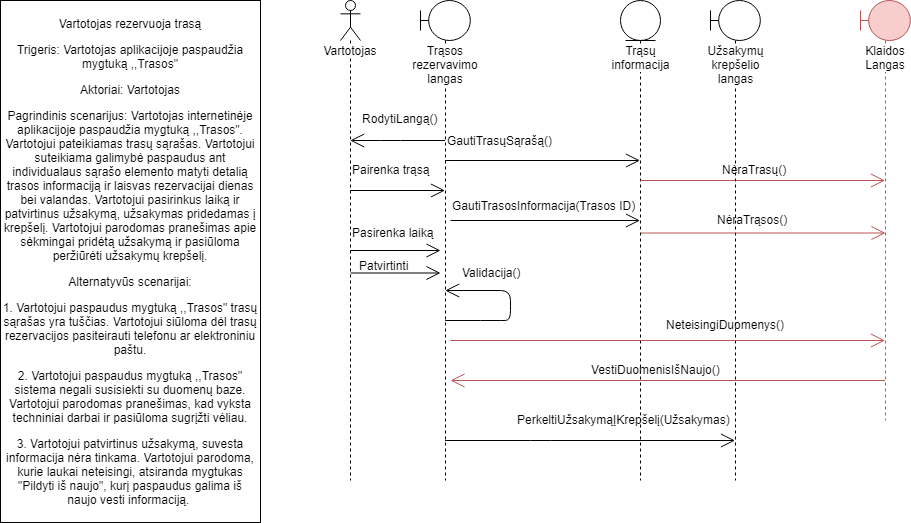
\includegraphics[width=1\textwidth]{seq8.png}
    				\caption{Vartotojas rezervuoja trasą}
    				\label{fig:VartotojoUseCasel}
			\end{figure}

			\begin{figure}[h]
    				\centering
    				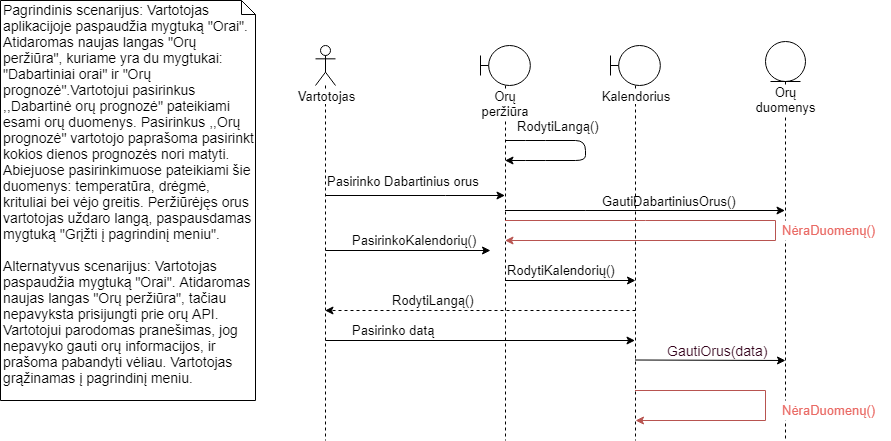
\includegraphics[width=1\textwidth]{seq10.png}
    				\caption{Vartotojas peržiūri orų prognozę}
    				\label{fig:Vartotojas peržiūri orų prognozę}
			\end{figure}

			\begin{figure}[h]
    				\centering
    				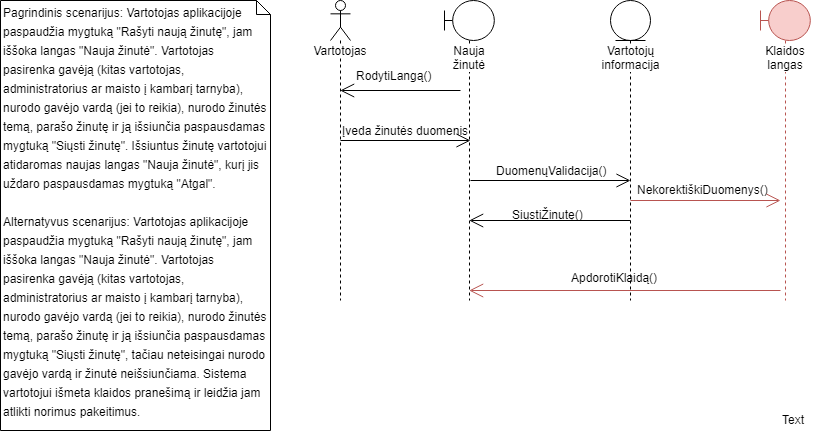
\includegraphics[width=1\textwidth]{seq11.png}
    				\caption{Vartotojas rašo žinutę}
    				\label{fig:Vartotojas rašo žinutę}
			\end{figure}

			\begin{figure}[h]
    				\centering
    				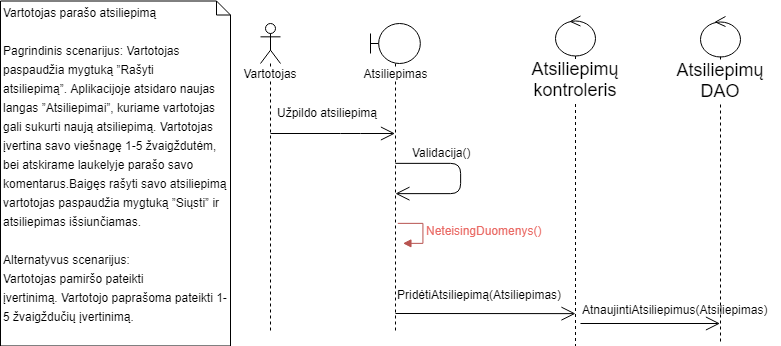
\includegraphics[width=1\textwidth]{seq12.png}
    				\caption{Vartotojas rašo atsiliepimą}
    				\label{fig:Vartotojas rašo atsiliepimą}
			\end{figure}

			\begin{figure}[h]
    				\centering
    				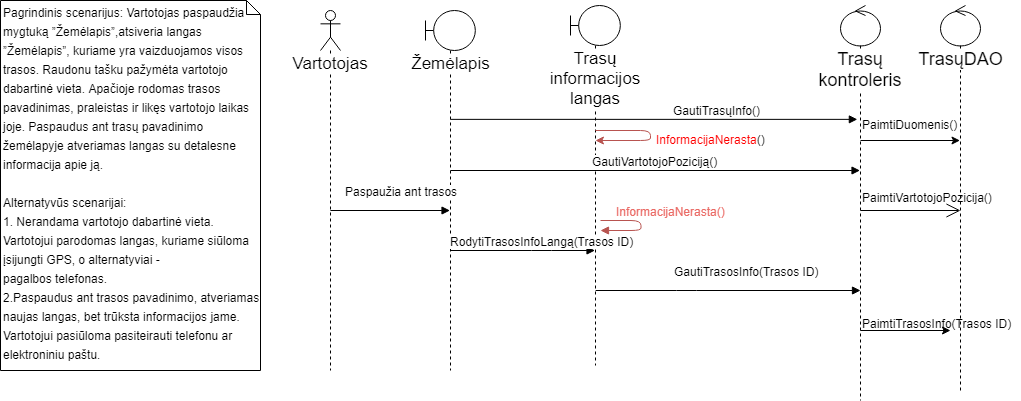
\includegraphics[width=1\textwidth]{seq13.png}
    				\caption{Vartotojas peržiūri žemėlapį}
    				\label{fig:Vartotojas peržiūri žemėlapį}
			\end{figure}

\section{Klasių diagrama}

			\begin{figure}[h]
    				\centering
    				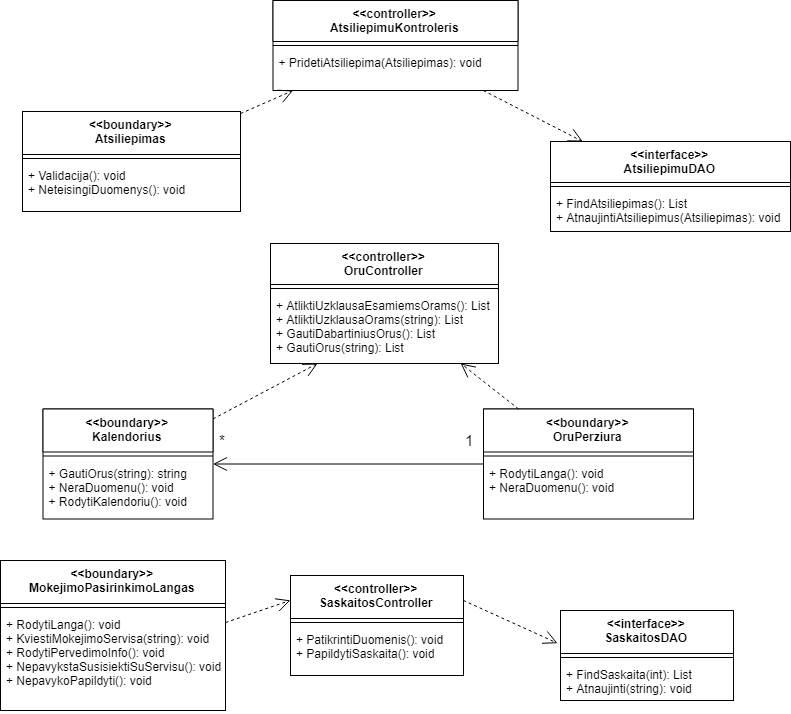
\includegraphics[width=1\textwidth]{classA.png}
    				\caption{Klasių diagrama 1}
    				\label{fig:KlasiuDiagrama}
			\end{figure}
			\begin{figure}[h]
    				\centering
    				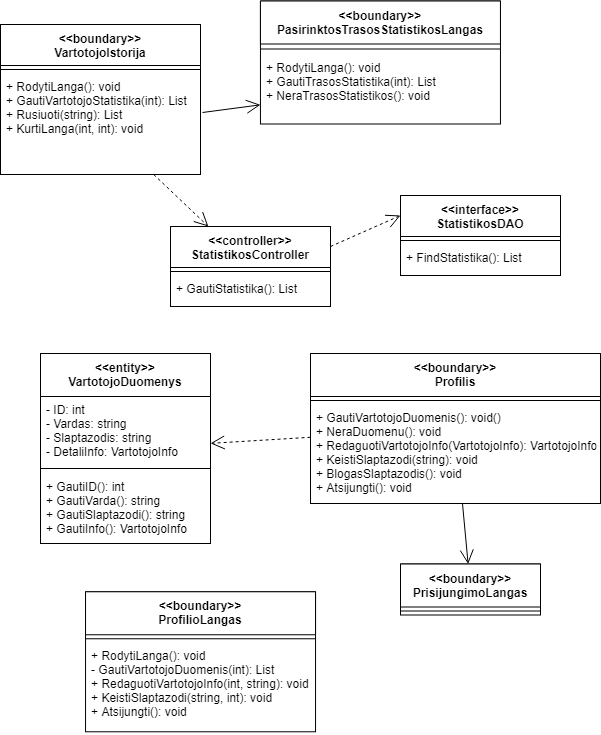
\includegraphics[width=1\textwidth]{classB.png}
    				\caption{Klasių diagrama 2}
    				\label{fig:KlasiuDiagrama}
			\end{figure}
			\begin{figure}[h]
    				\centering
    				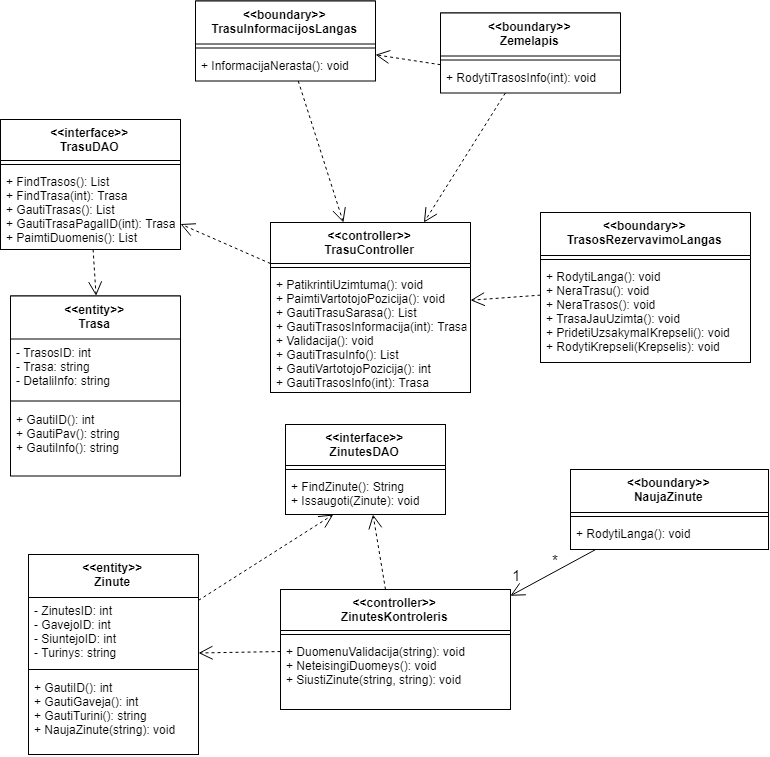
\includegraphics[width=1\textwidth]{classC.png}
    				\caption{Klasių diagrama 3}
    				\label{fig:KlasiuDiagrama}
			\end{figure}
			\begin{figure}[h]
    				\centering
    				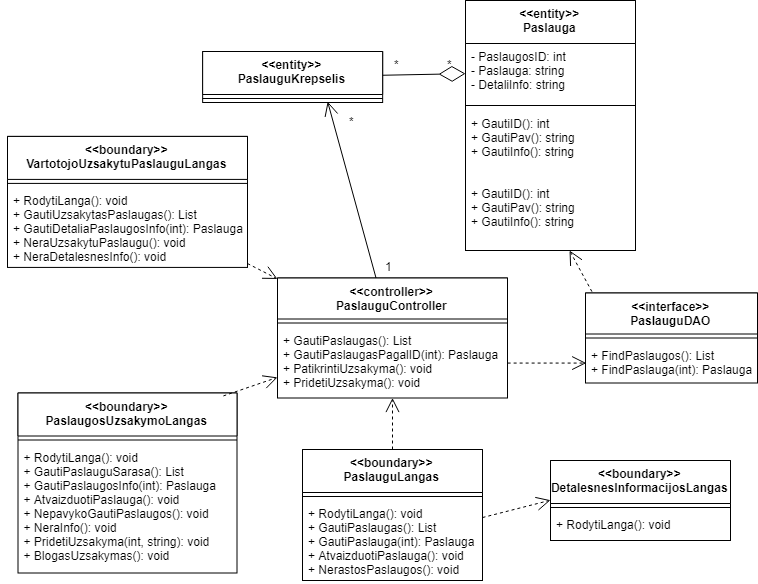
\includegraphics[width=1\textwidth]{classD.png}
    				\caption{Klasių diagrama 4}
    				\label{fig:KlasiuDiagrama}
			\end{figure}

\section{Detalaus projekto peržiūra}
	\subsection{Peržiūra}
Peržiūros metu sutvarkėme savo robastiškumo ir sekų diagramas, kad jos atitiktų viena kitą ir atitiktų use case'us. Pridėjome papildomus alternatyvius scenarijus. Pagrindinis dalykas, kurį pakeitėm yra atskiras langas, kuris atsiranda įvykus nenumatytam scenarijui. Dabar pagal sekų diagramas įvykus alternatyviam scenarijui informacinė žinutė atsiranda tame pačiame lange, kuris buvo atsakingas dėl sukeltos klaidos.  Ištrynėme nereikalingus kontrolerius, kurie nieko nedarė. Panaikinome ,,Ataskaitos" use case'a, nes supratome, kad šis use case'as yra neaiškus ir geriau pagalvojus nebūtinas mūsų sistemai funkcionuoti. Pagal pakeistas sekų diagramas taip pat pakeitėme klasių diagramą. Po peržiūros esame pasiruošę pradėti rašyti kodą. Peržiūrą vykdėme dviem etapais. Pirmame etame kiekvienas komandos narys peržiūrėjo tas diagramas, kurių jis nedarė(svetimas klaidas pastebėti lengviau). Antrame etape susirinko visa komanda ir ėjome po vieną  diagramą aptardami, ar viskas joje gerai, ir padarydami paskutinius pataisymus.
	\subsection{Atsekamumas}
	
	\begin{figure}[h]
    				\centering
    				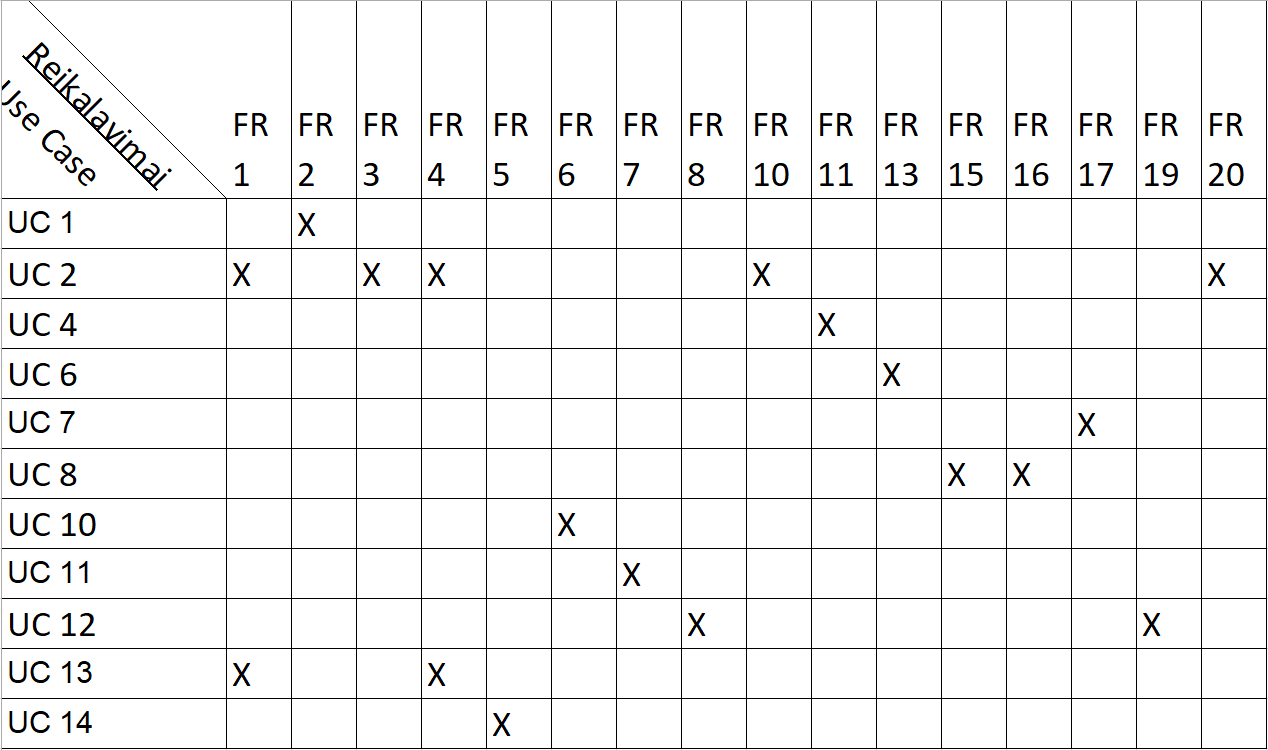
\includegraphics[width=0.75\textwidth]{UCxFR.png}
    				\caption{UC - FR atsekamumas}
			\end{figure}
			
	\begin{figure}[h]
    				\centering
    				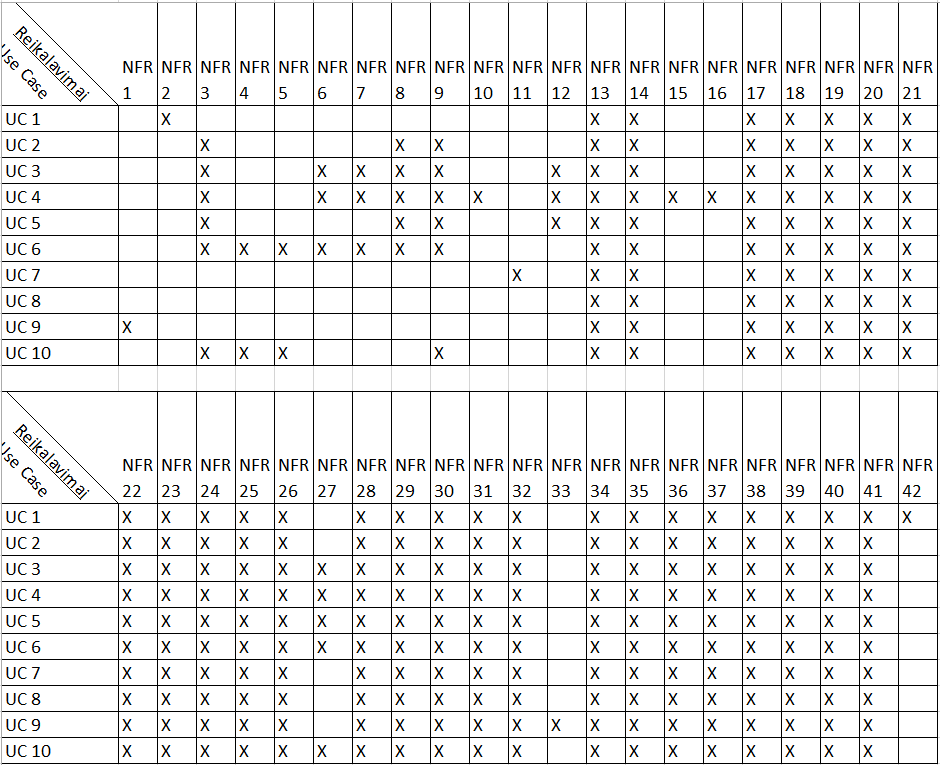
\includegraphics[width=1\textwidth]{UC_NFR.png}
    				\caption{UC - NFR atsekamumas}
			\end{figure}
\section{Testavimo scenarijai}
	
			\begin{figure}[h]
    				\centering
    				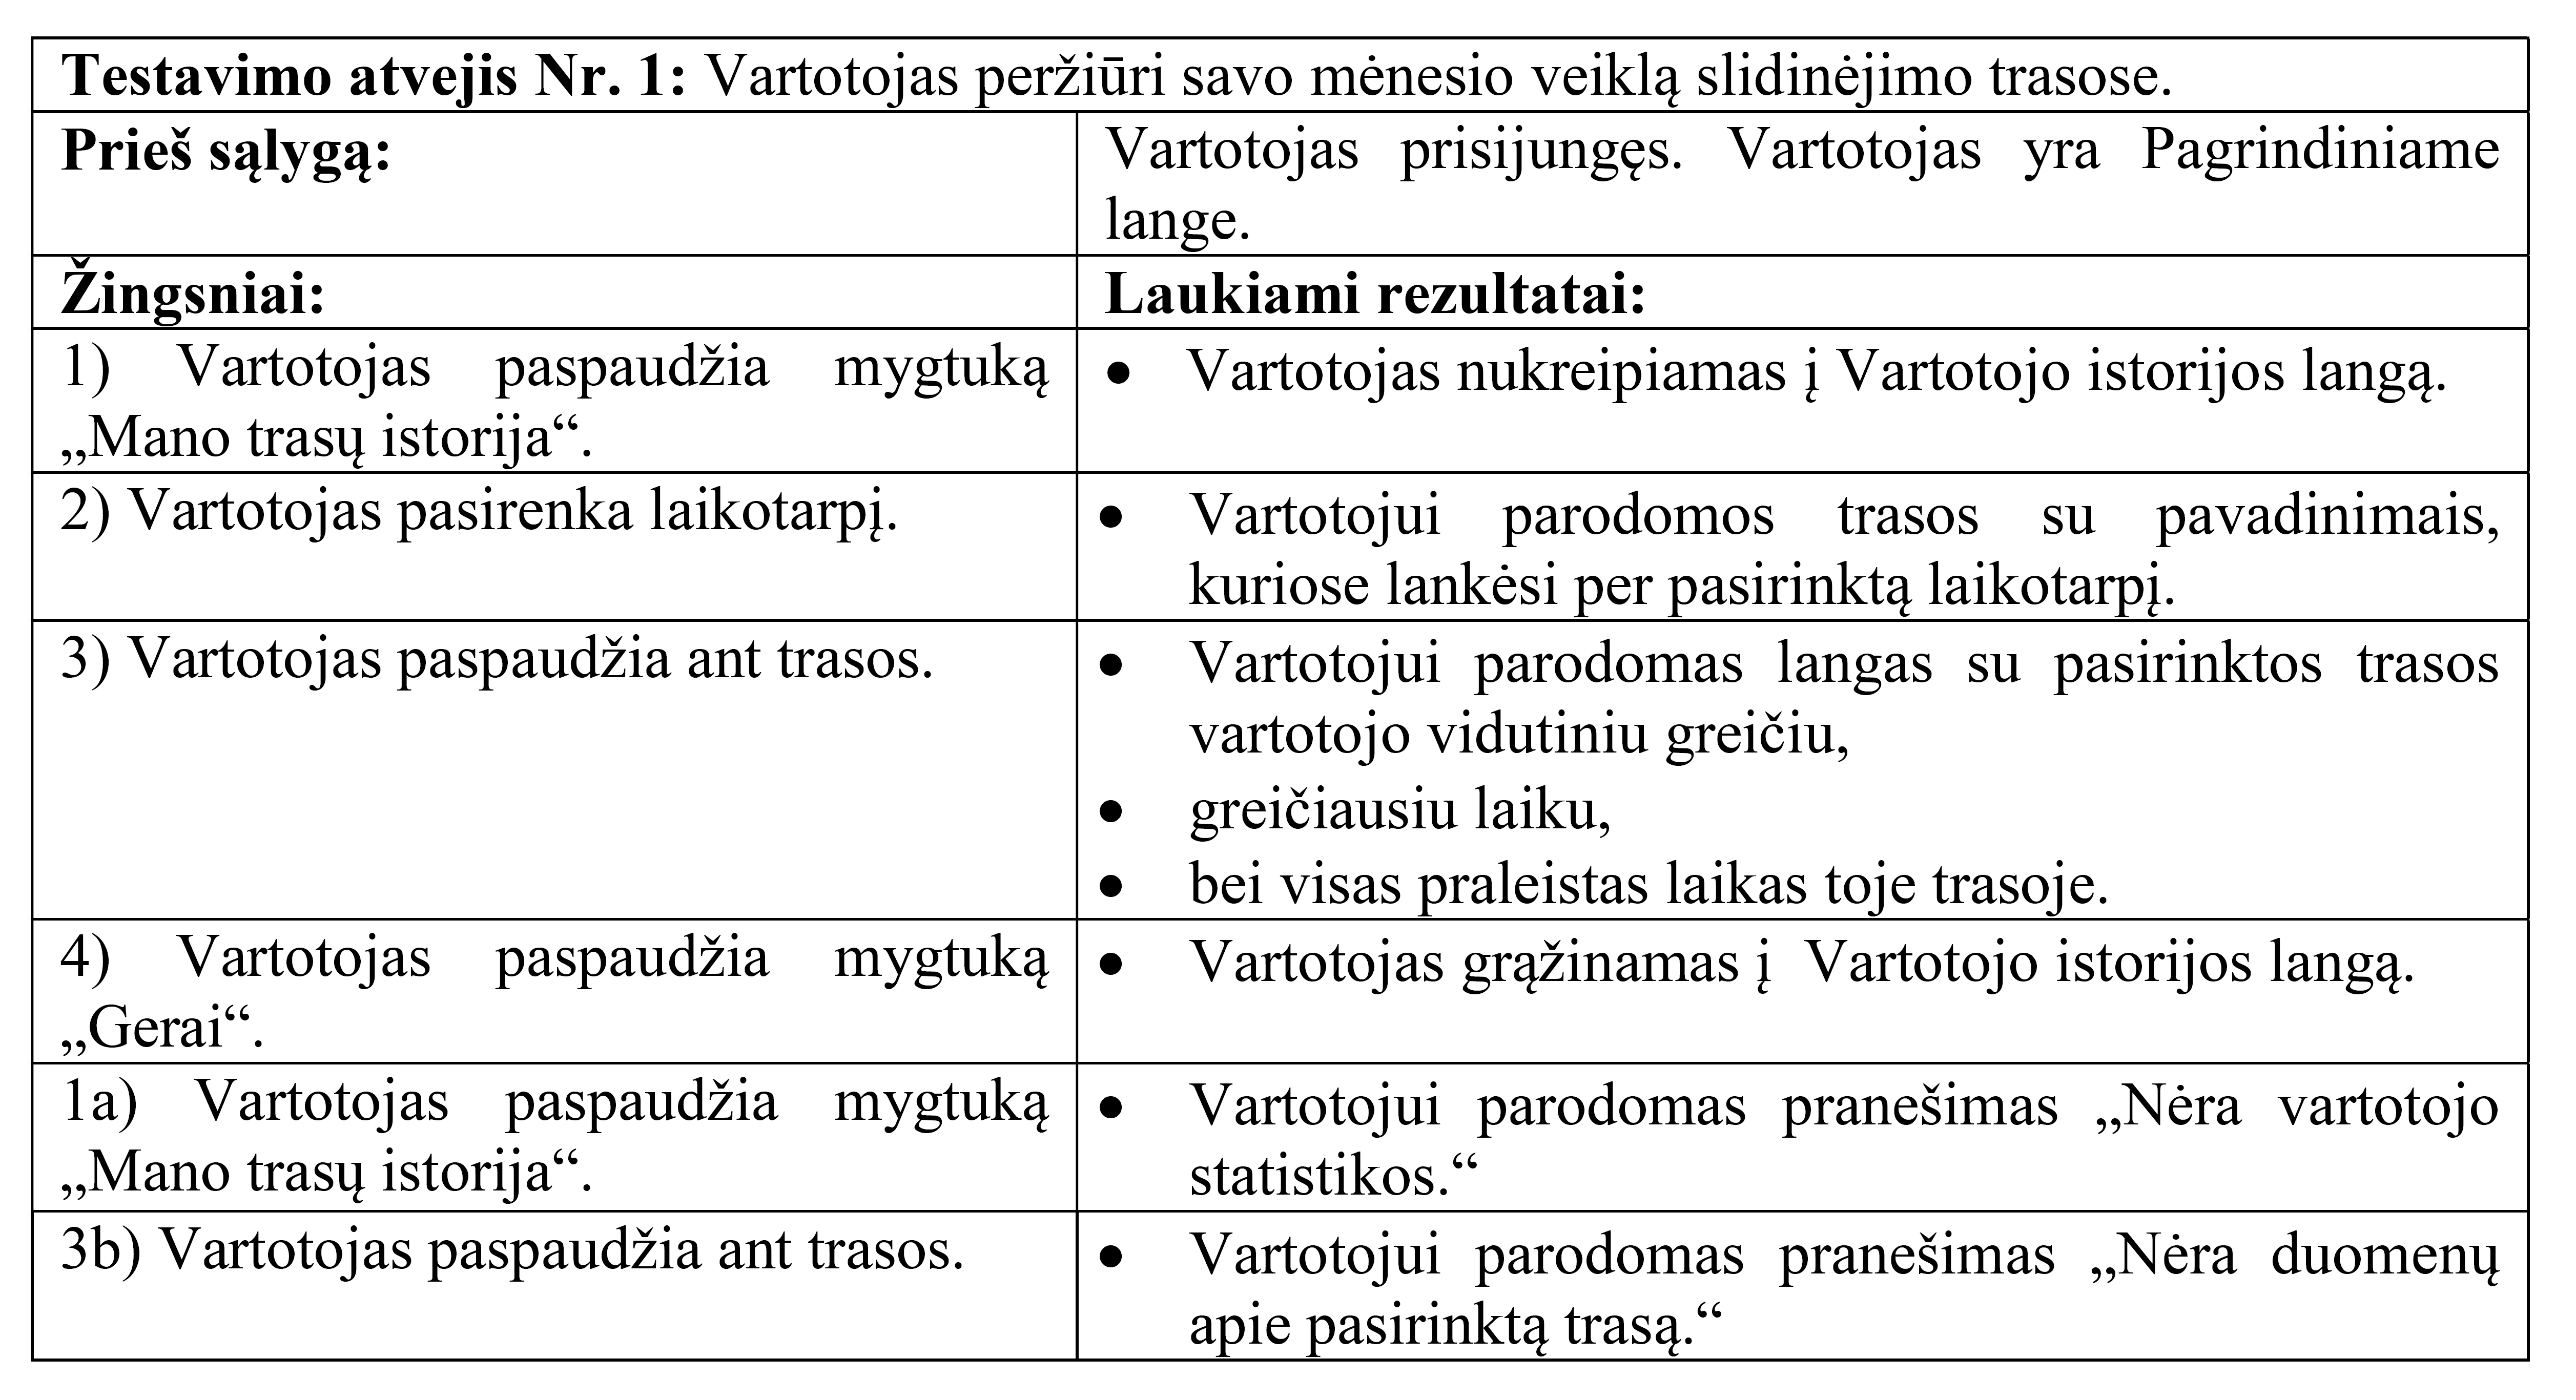
\includegraphics[width=1\textwidth]{test1.png}
    				\caption{Testas: Vartotojas peržiūri savo mėnesio veiklą}
    				\label{fig:Testas: Vartotojas peržiūri savo mėnesio veiklą}
			\end{figure}
			
			\begin{figure}[h]
    				\centering
    				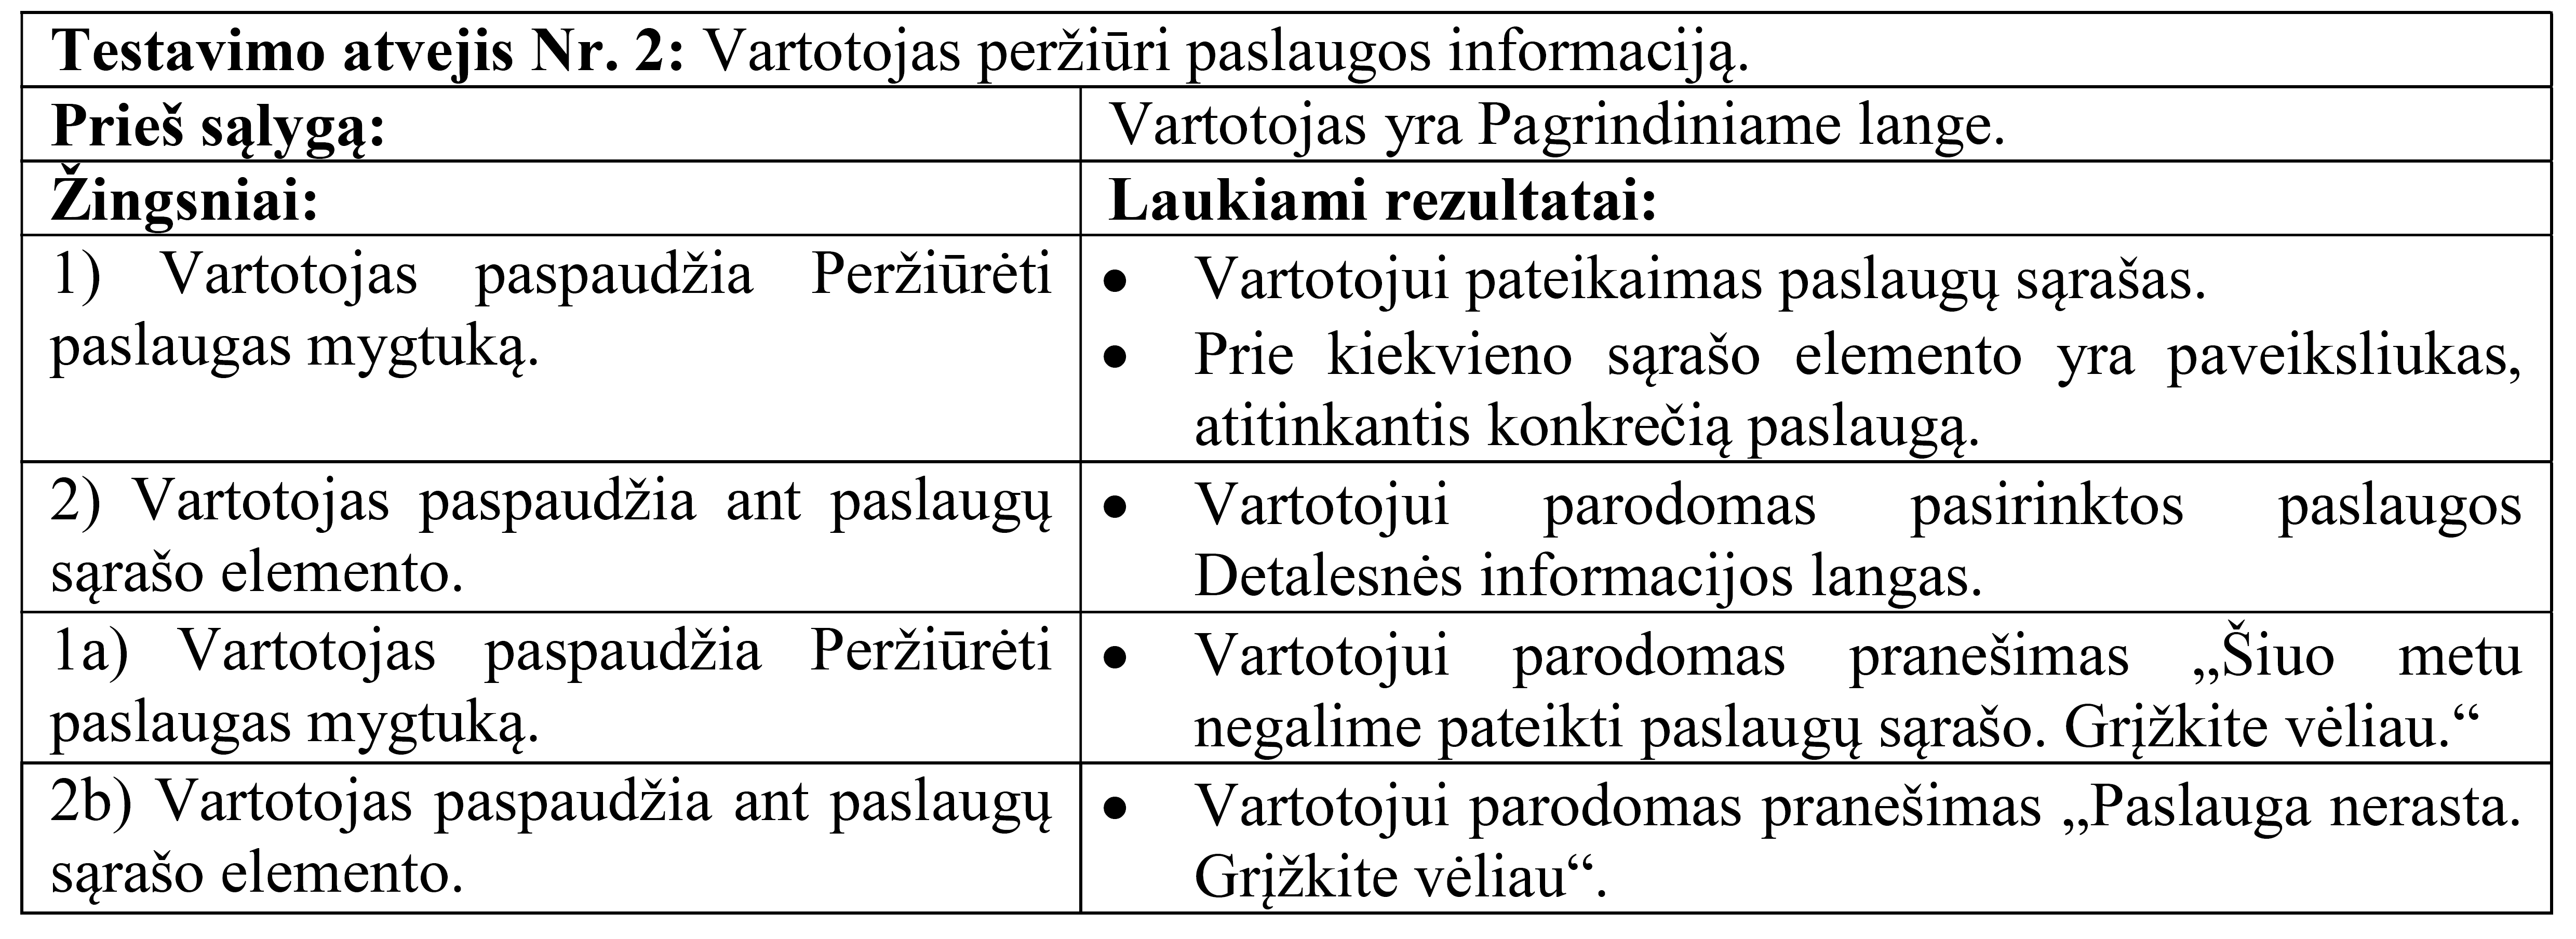
\includegraphics[width=1\textwidth]{test2.png}
    				\caption{Testas: Vartotojas peržiūri paslaugos informaciją}
    				\label{fig:Testas: Vartotojas peržiūri paslaugos informaciją}
			\end{figure}
			
			\begin{figure}[h]
    				\centering
    				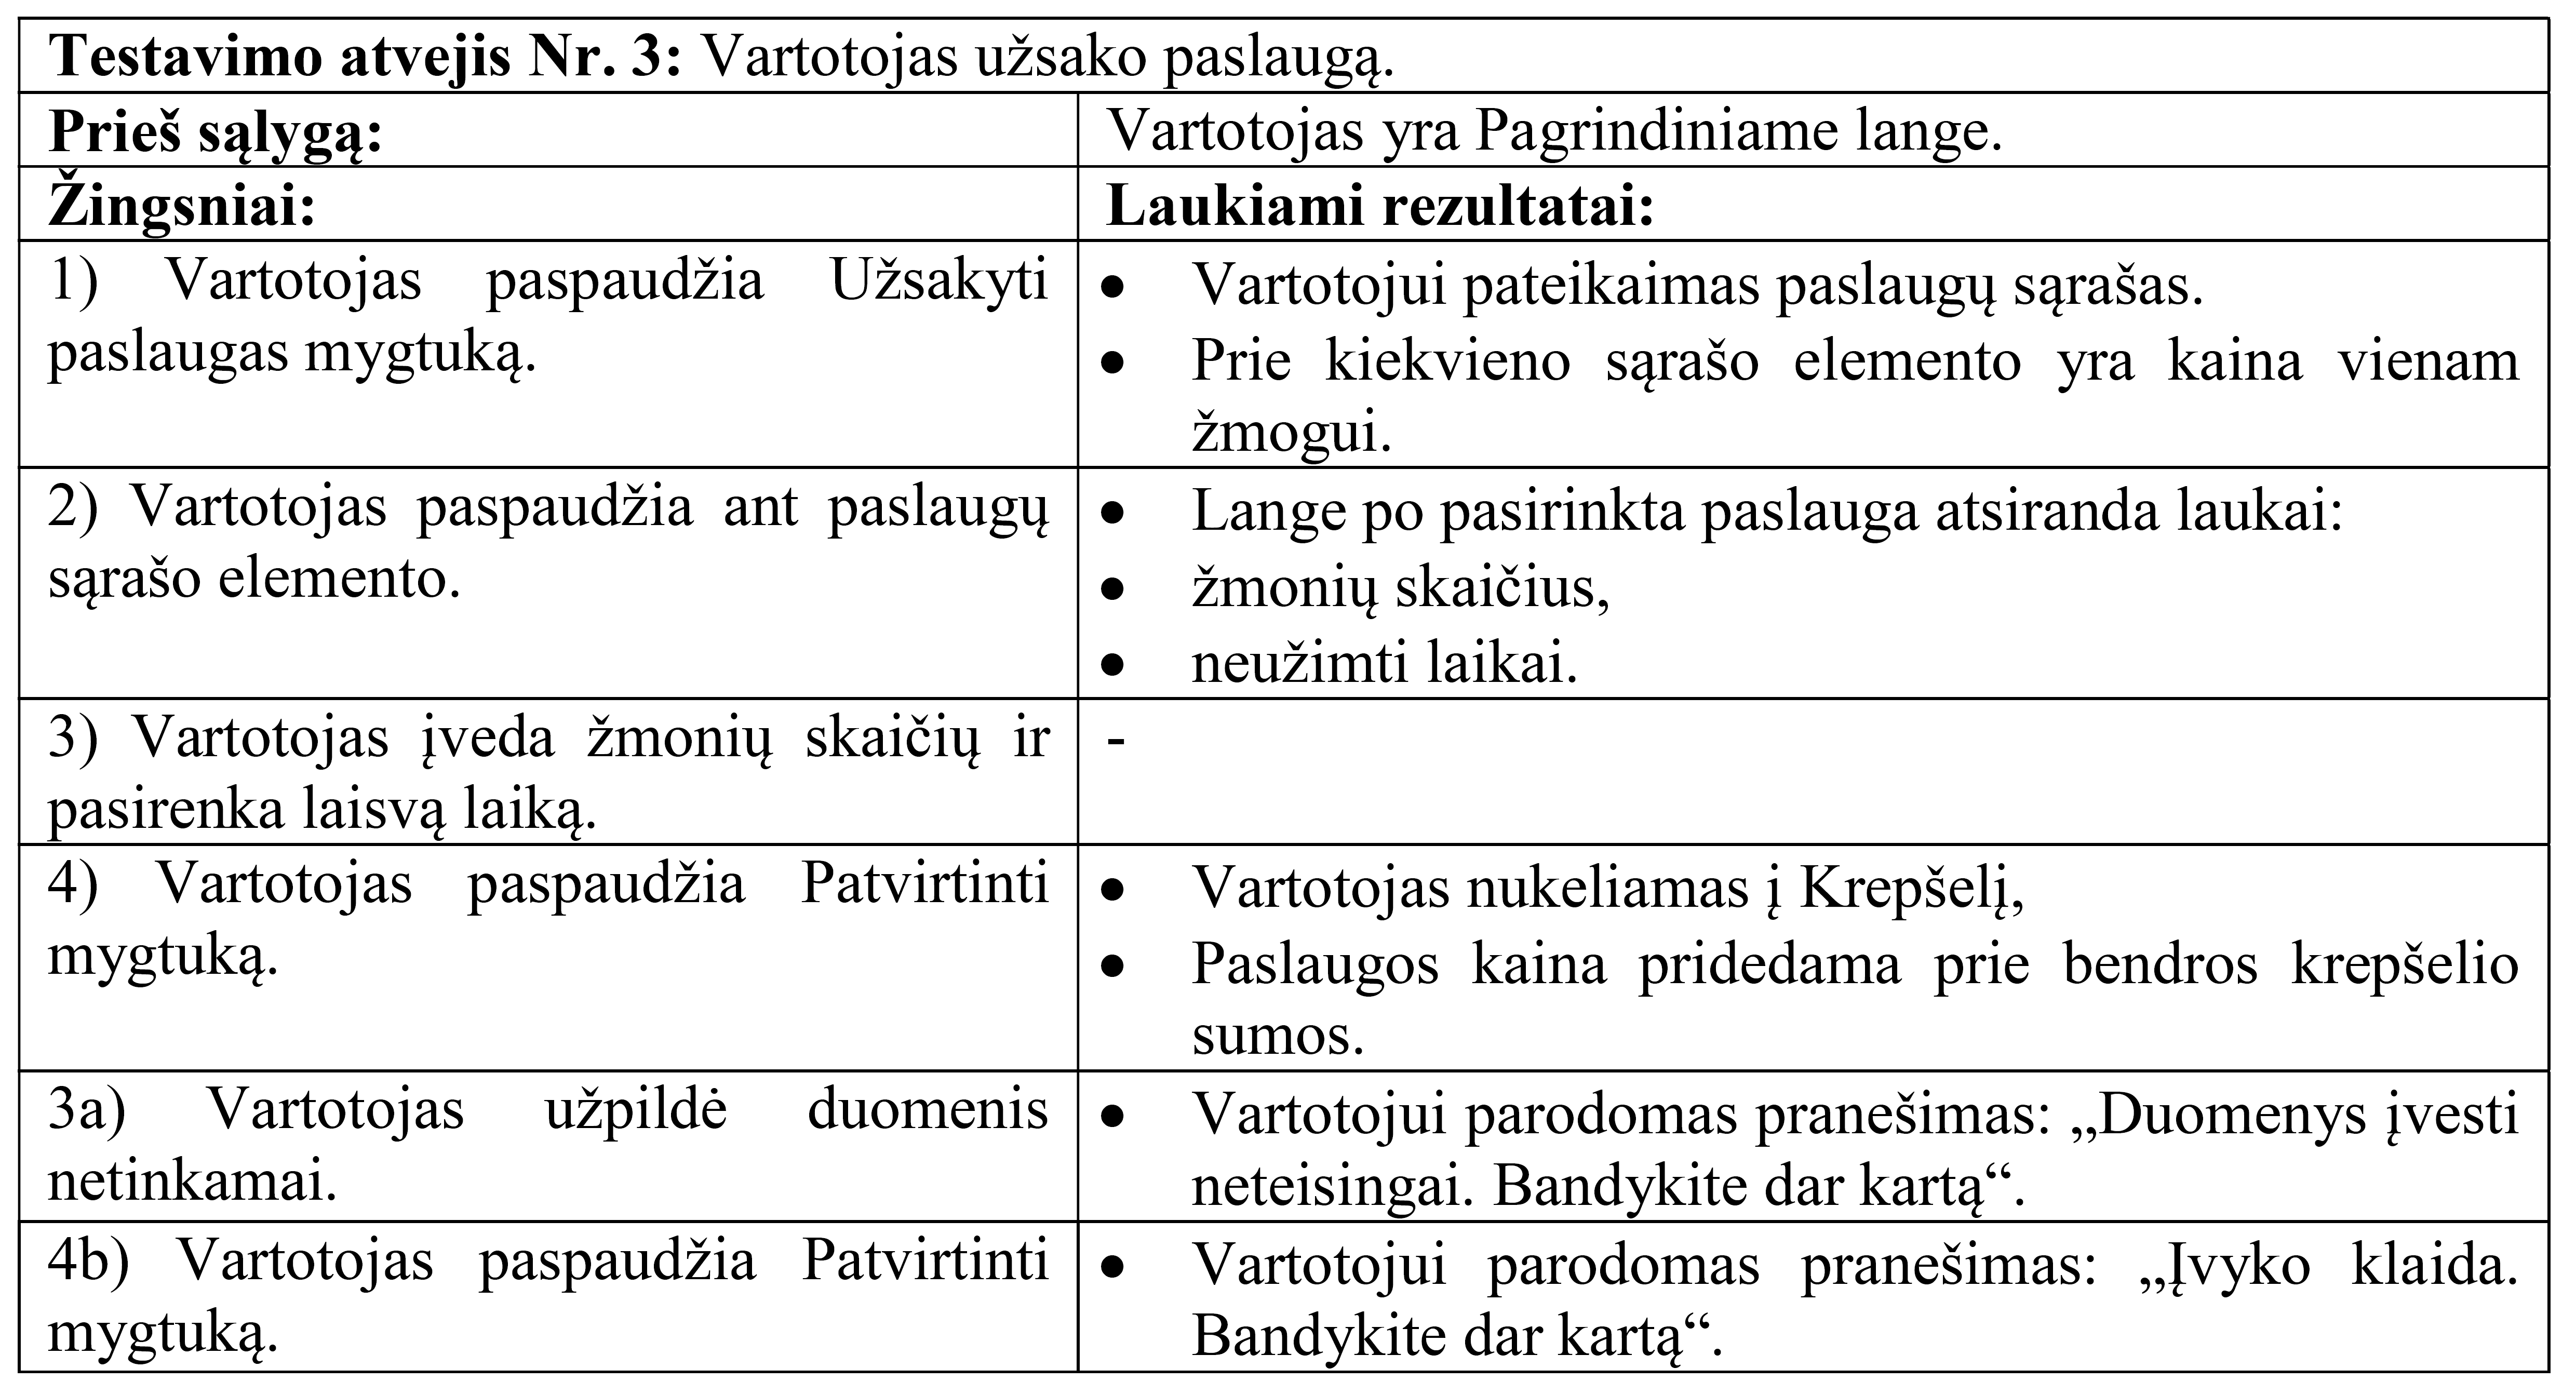
\includegraphics[width=1\textwidth]{test3.png}
    				\caption{Testas: Vartotojas užsako paslaugą}
    				\label{fig:Testas: Vartotojas užsako paslaugą}
			\end{figure}
			
			\begin{figure}[h]
    				\centering
    				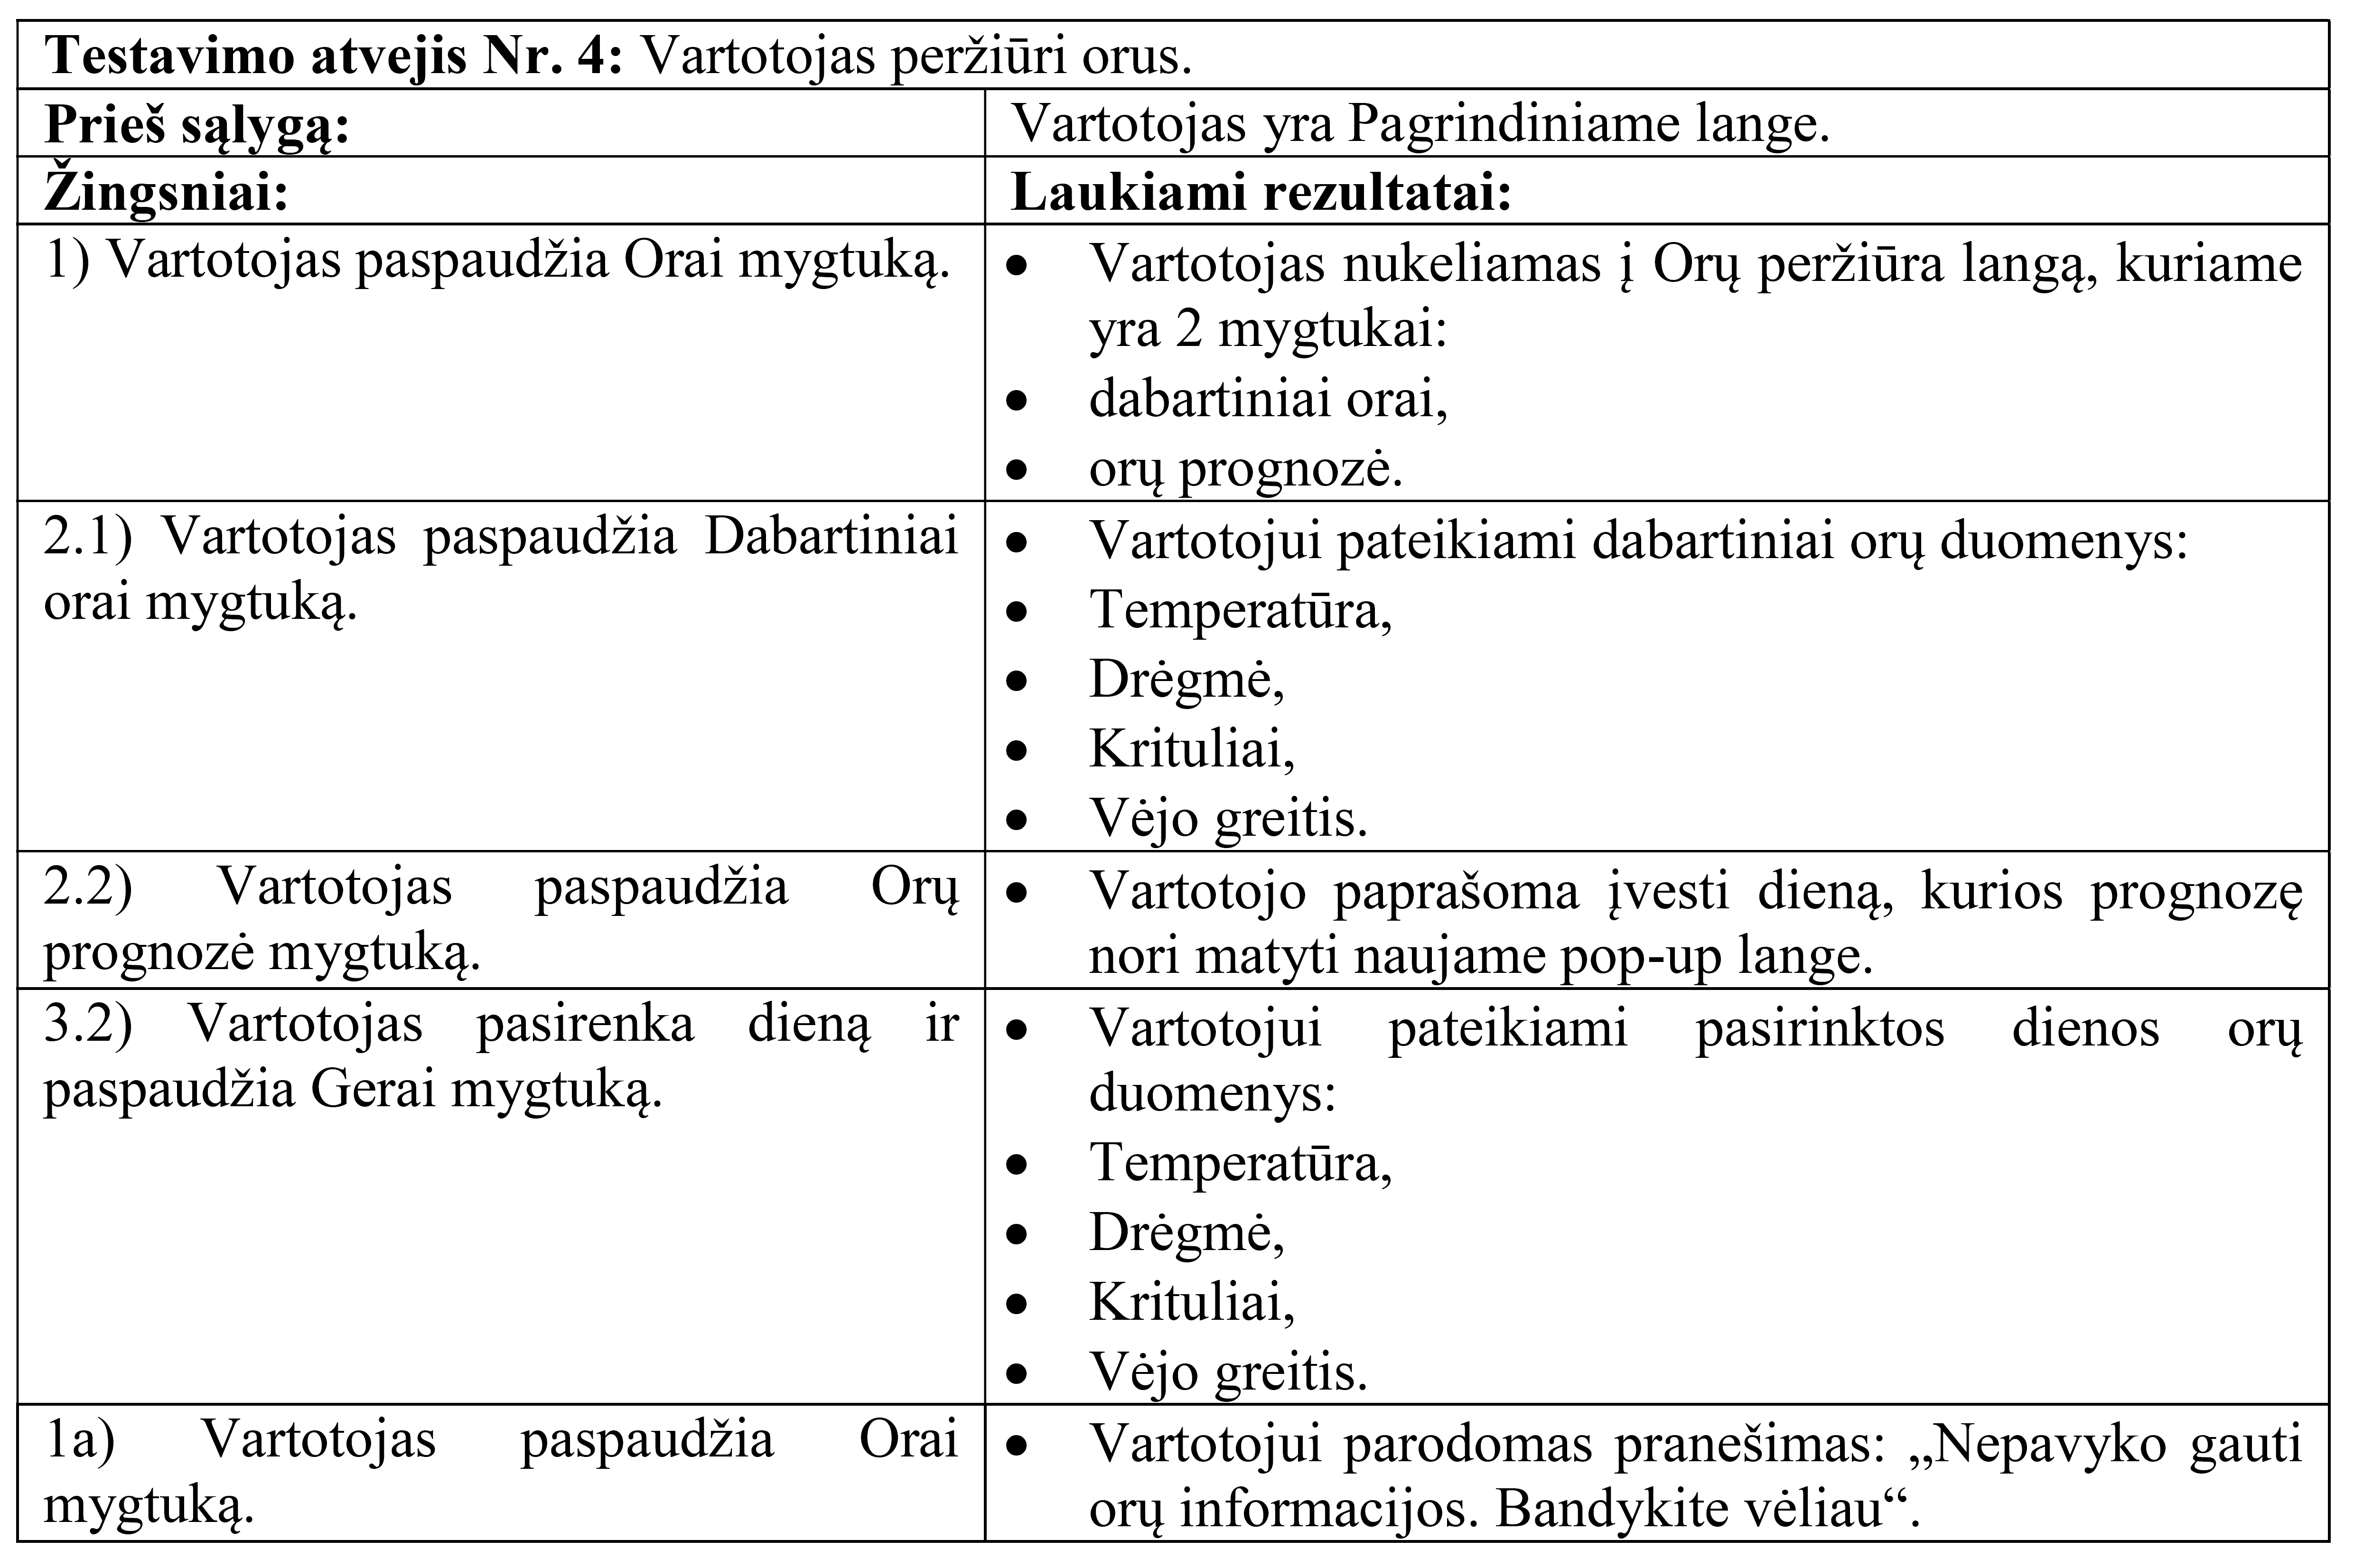
\includegraphics[width=1\textwidth]{test4.png}
    				\caption{Testas: Vartotojas peržiūri orus}
    				\label{fig:Testas: Vartotojas peržiūri orus}
			\end{figure}
			
			\begin{figure}[h]
    				\centering
    				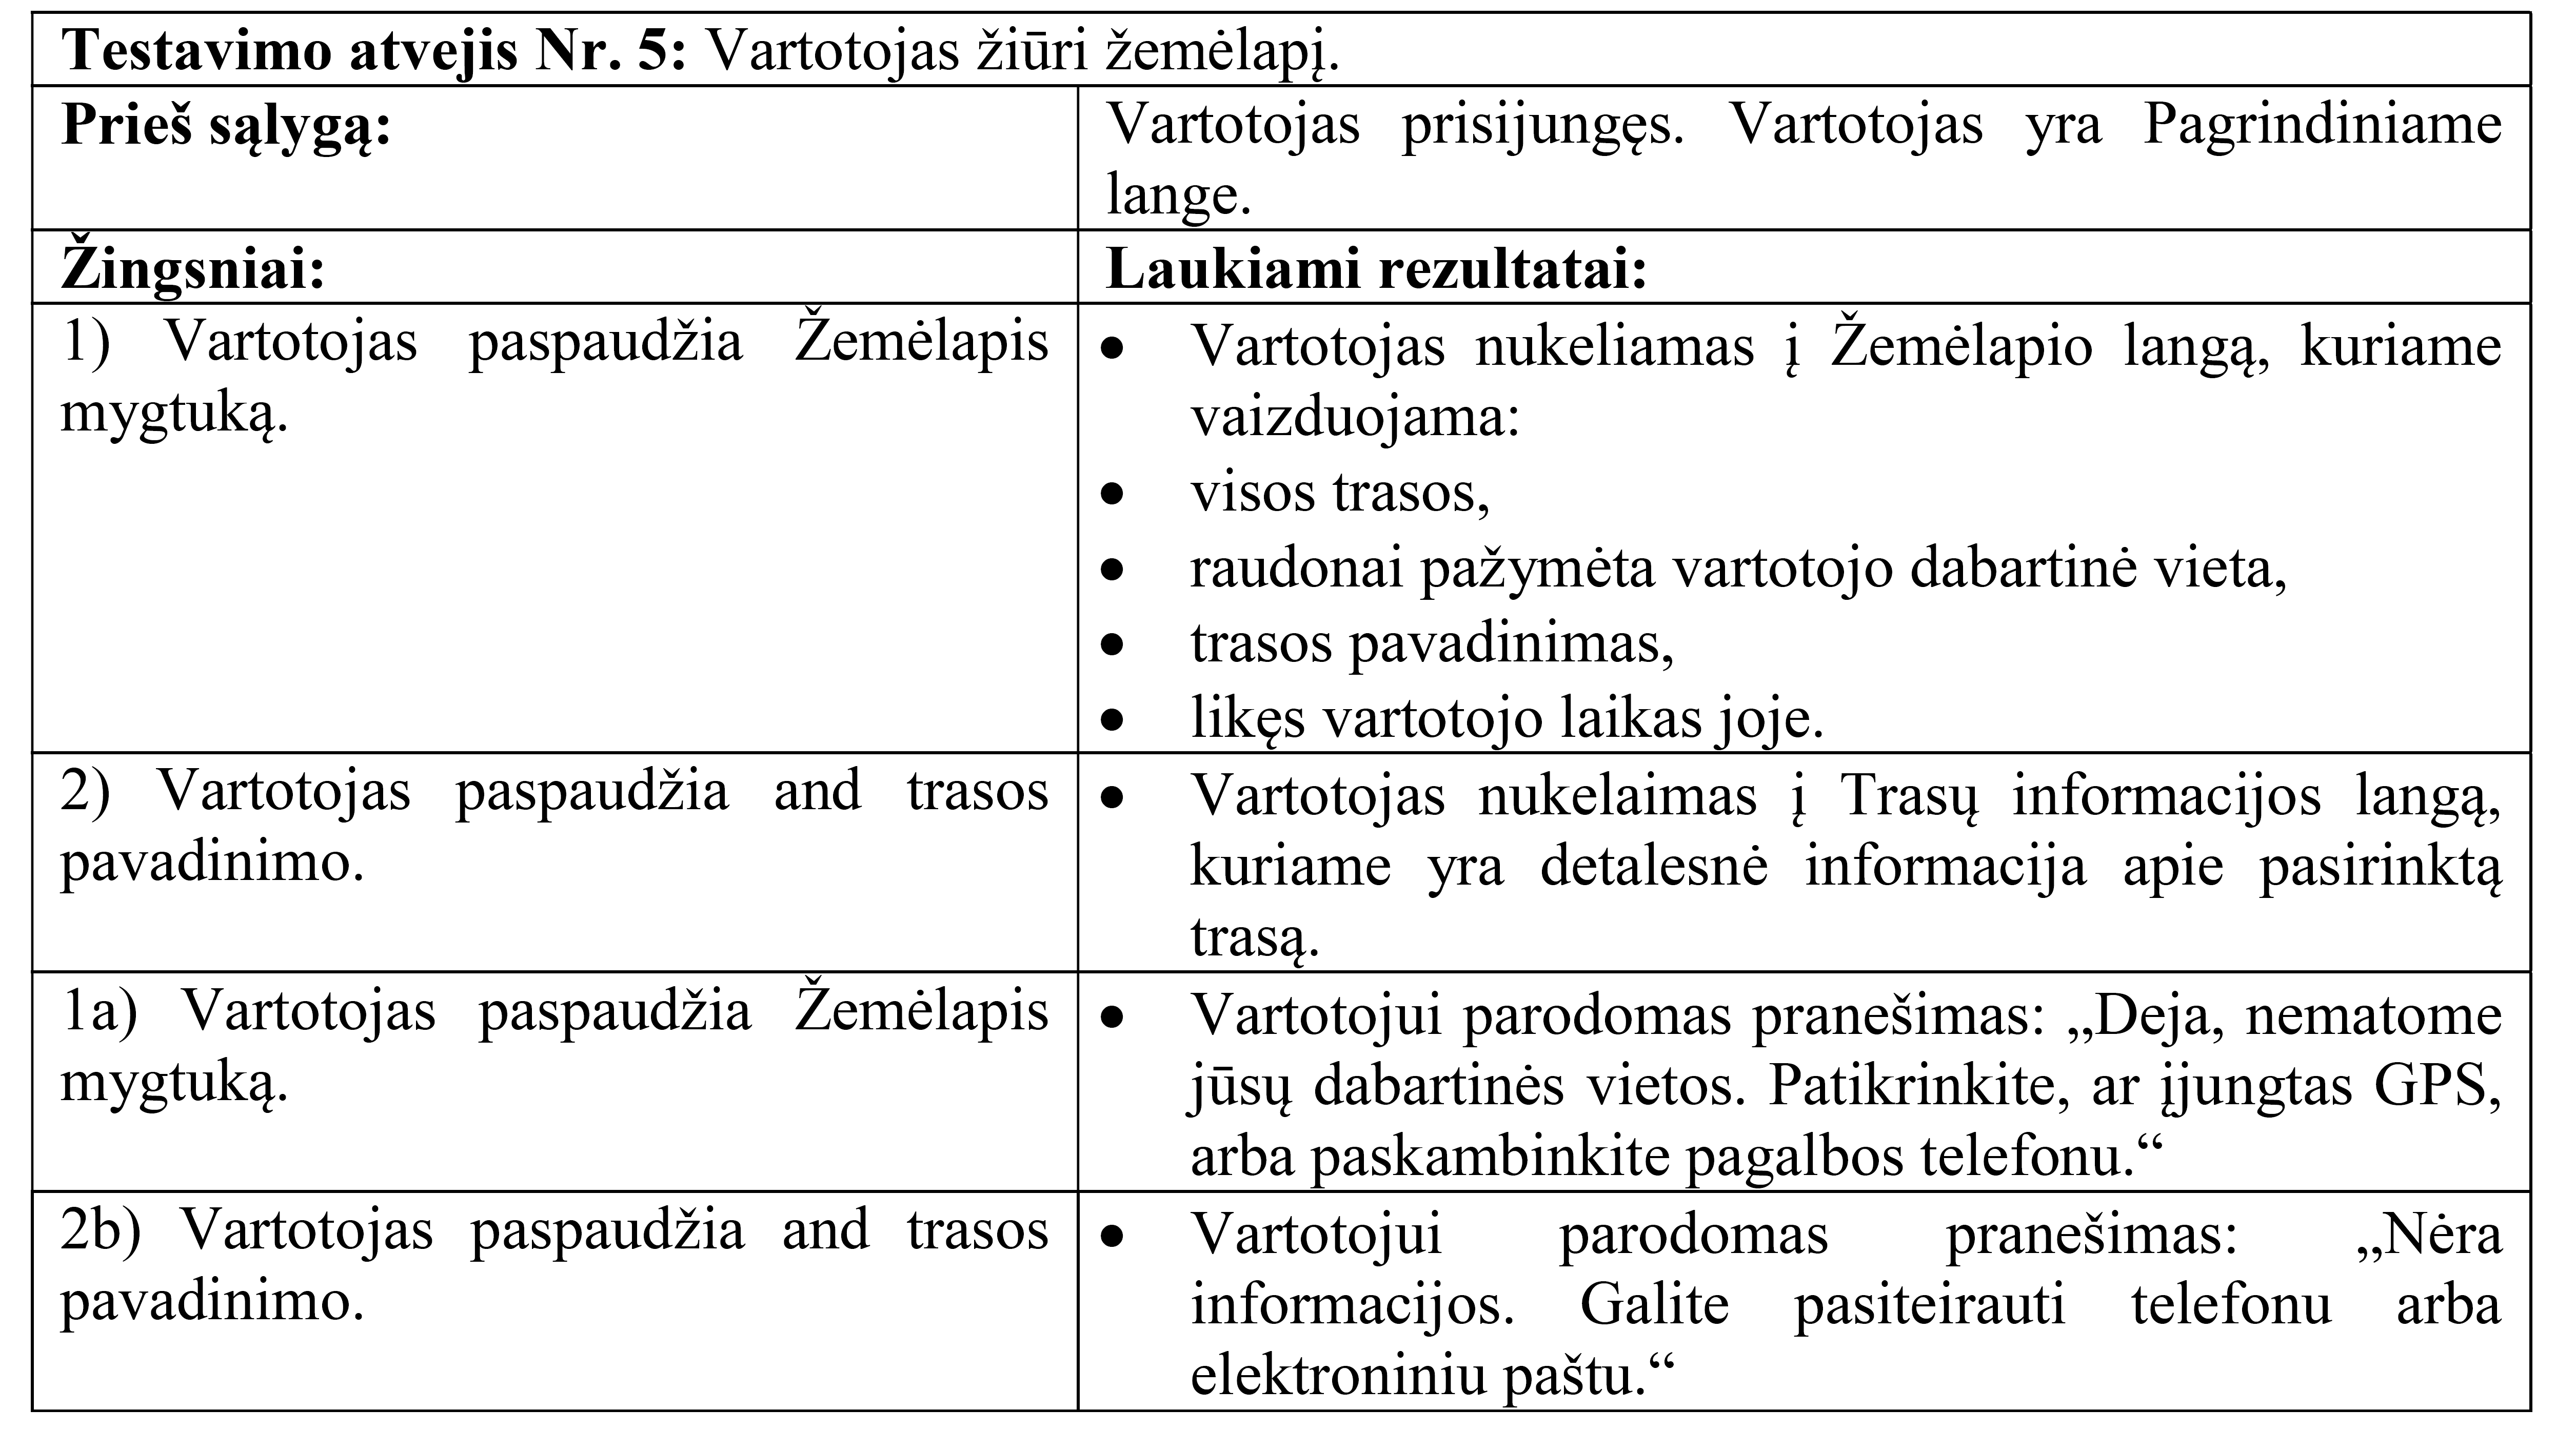
\includegraphics[width=1\textwidth]{test5.png}
    				\caption{Testas: Vartotojas žiūri žemėlapį}
    				\label{fig:Testas: Vartotojas žiūri žemėlapį}
			\end{figure}
			
			\begin{figure}[h]
    				\centering
    				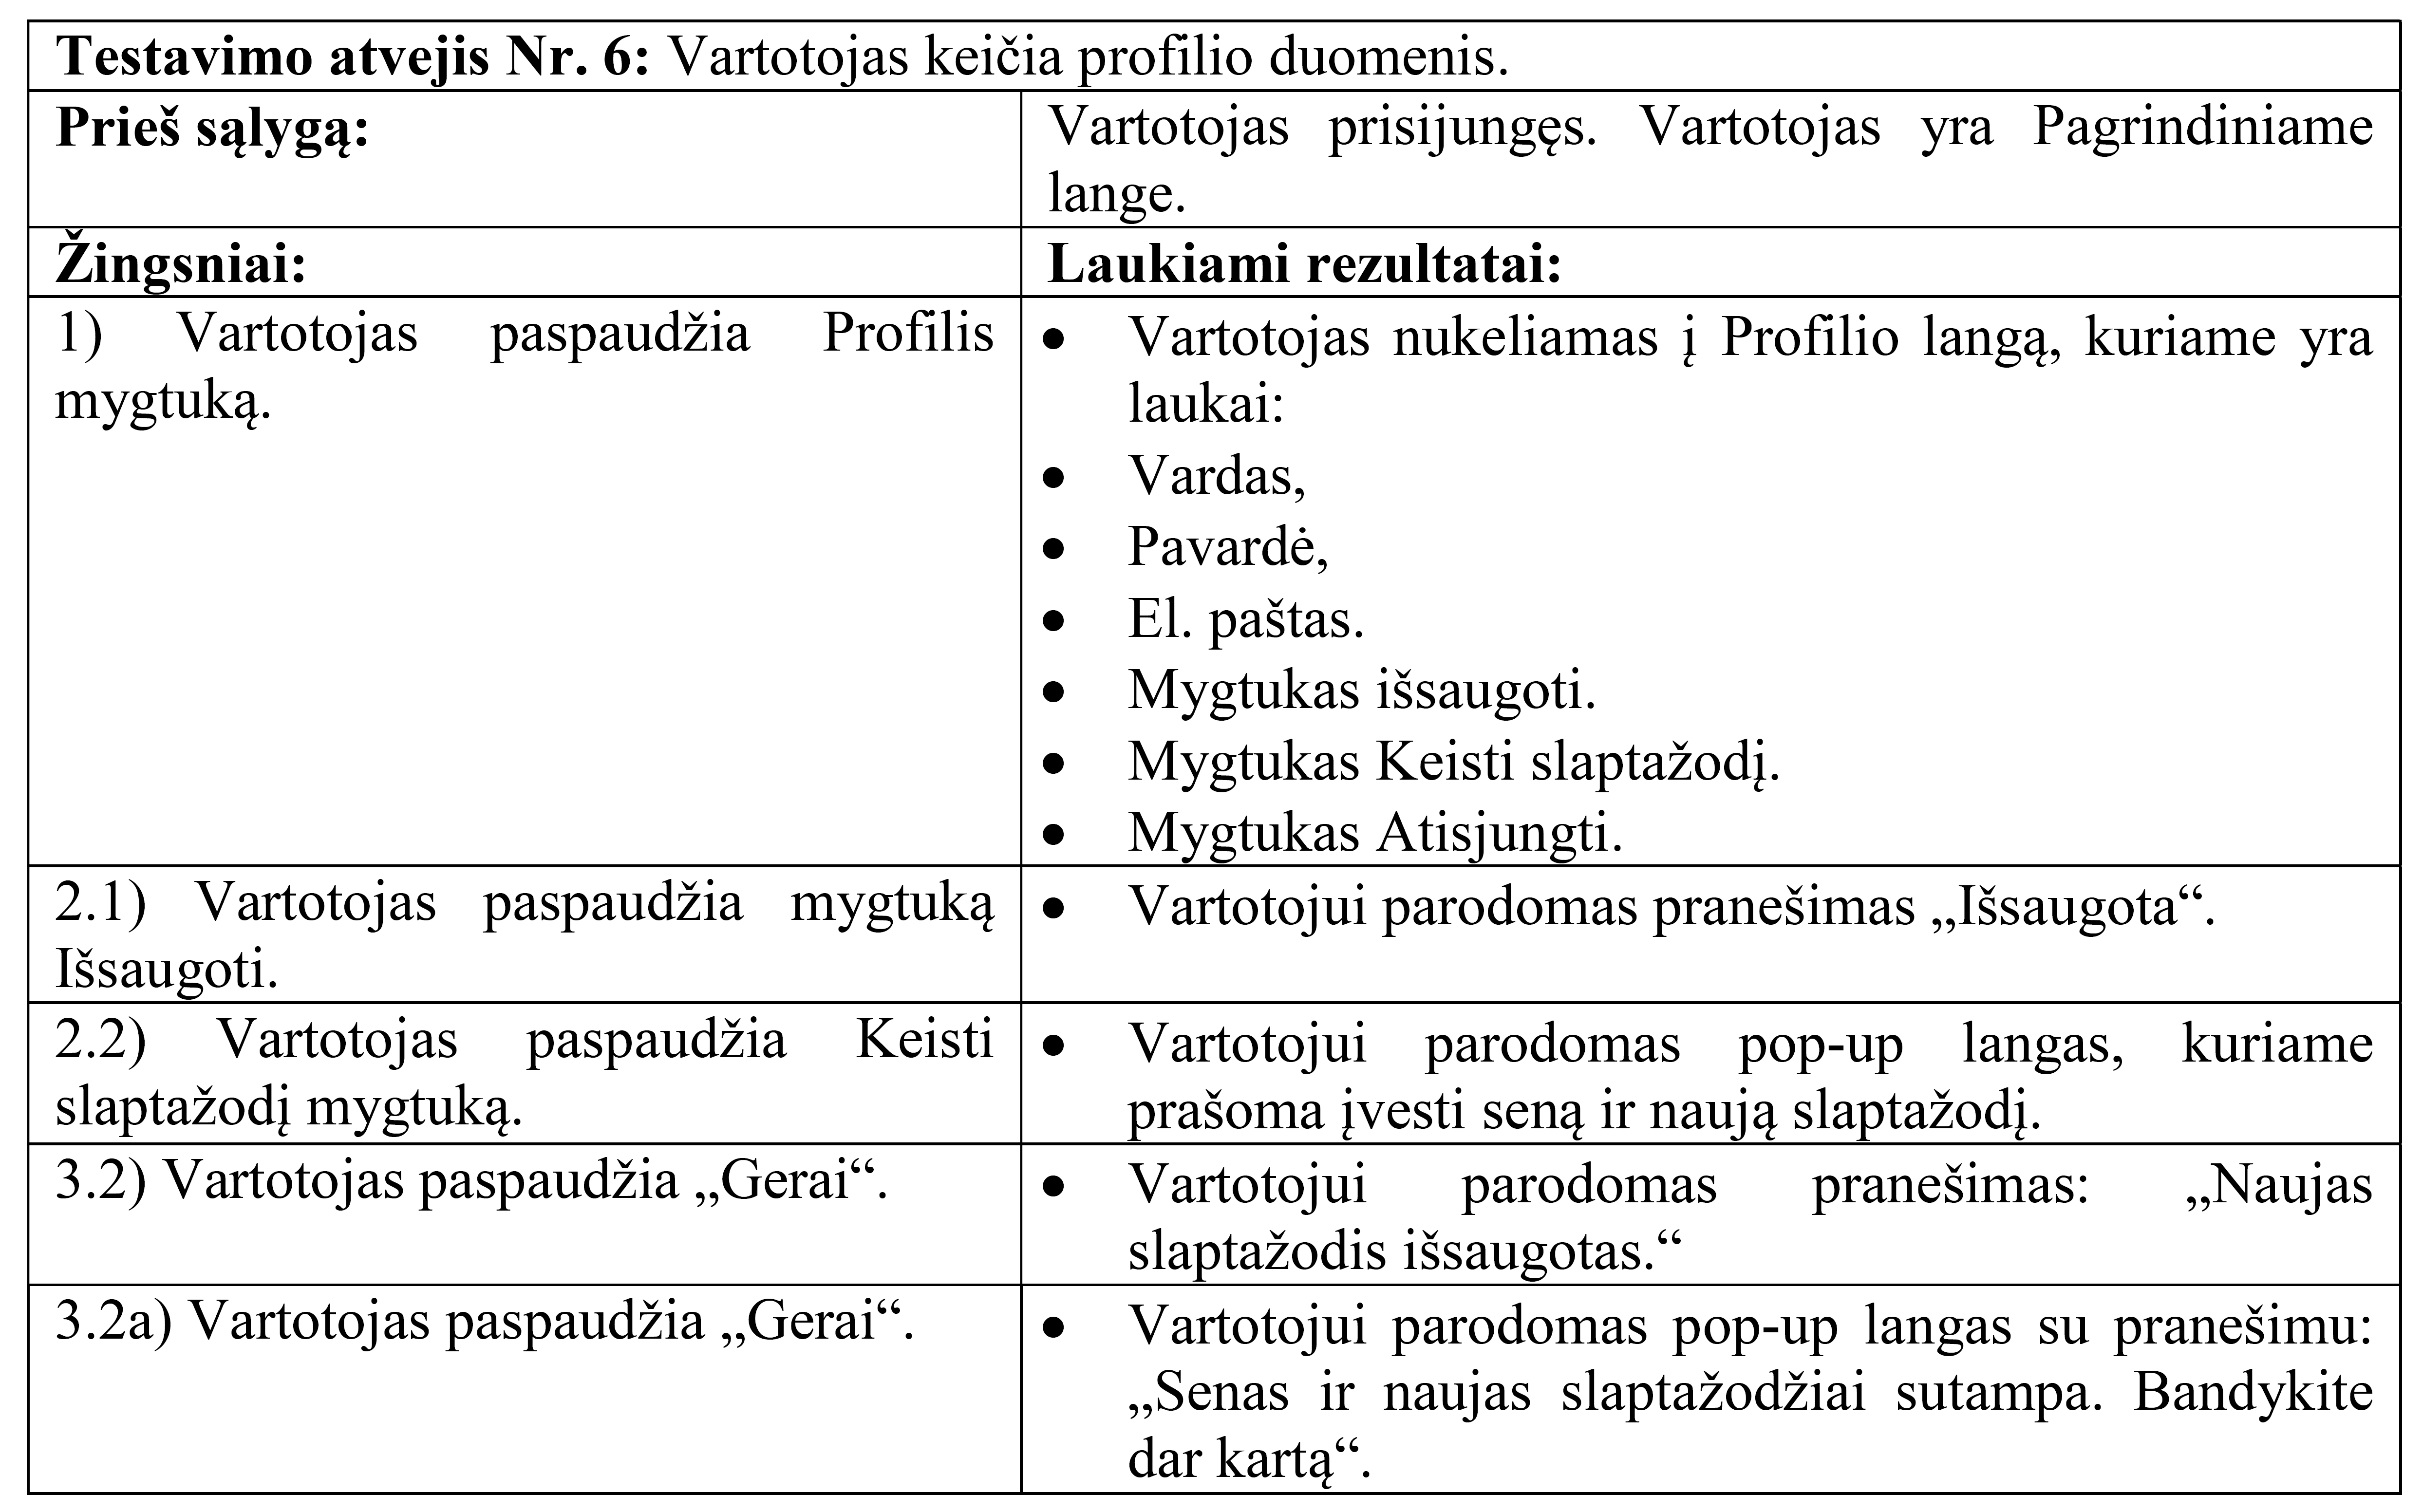
\includegraphics[width=1\textwidth]{test6.png}
    				\caption{Testas: Vartotojas keičia profilio duomenis}
    				\label{fig:Testas: Vartotojas keičia profilio duomenis}
			\end{figure}

			\begin{figure}[h]
    				\centering
    				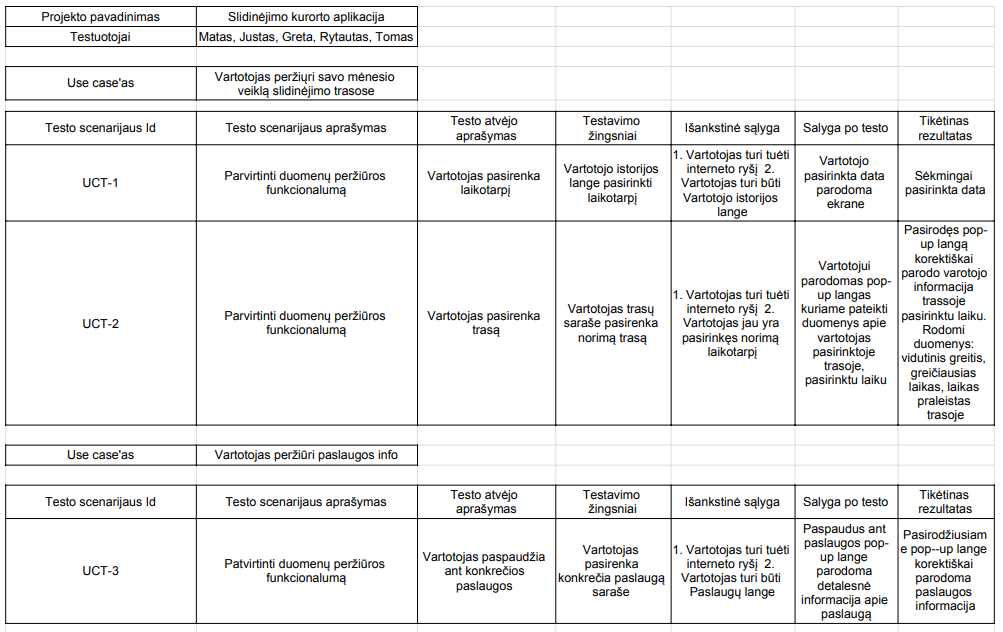
\includegraphics[width=1\textwidth]{testPlanPartOne.png}
    				\caption{Testas: Papildomas testavimo planas}
    				\label{fig:Testas:Papildomas testavimo planas}
			\end{figure}

			\begin{figure}[h]
    				\centering
    				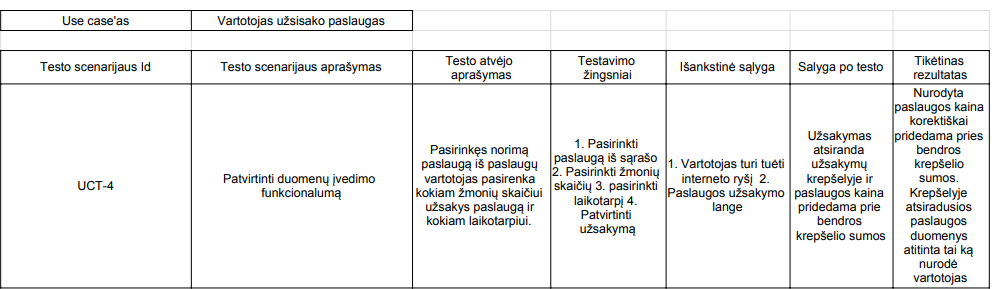
\includegraphics[width=1\textwidth]{testPlanPartTwo.png}
    				\caption{Testas: Papildomas testavimo planas}
    				\label{fig:Testas:Papildomas testavimo planas}
			\end{figure}

\section{Sistemos techninė architektūra}
	\subsection{Sistemos komponentų diagrama}
			\begin{figure}[h]
    				\centering
    				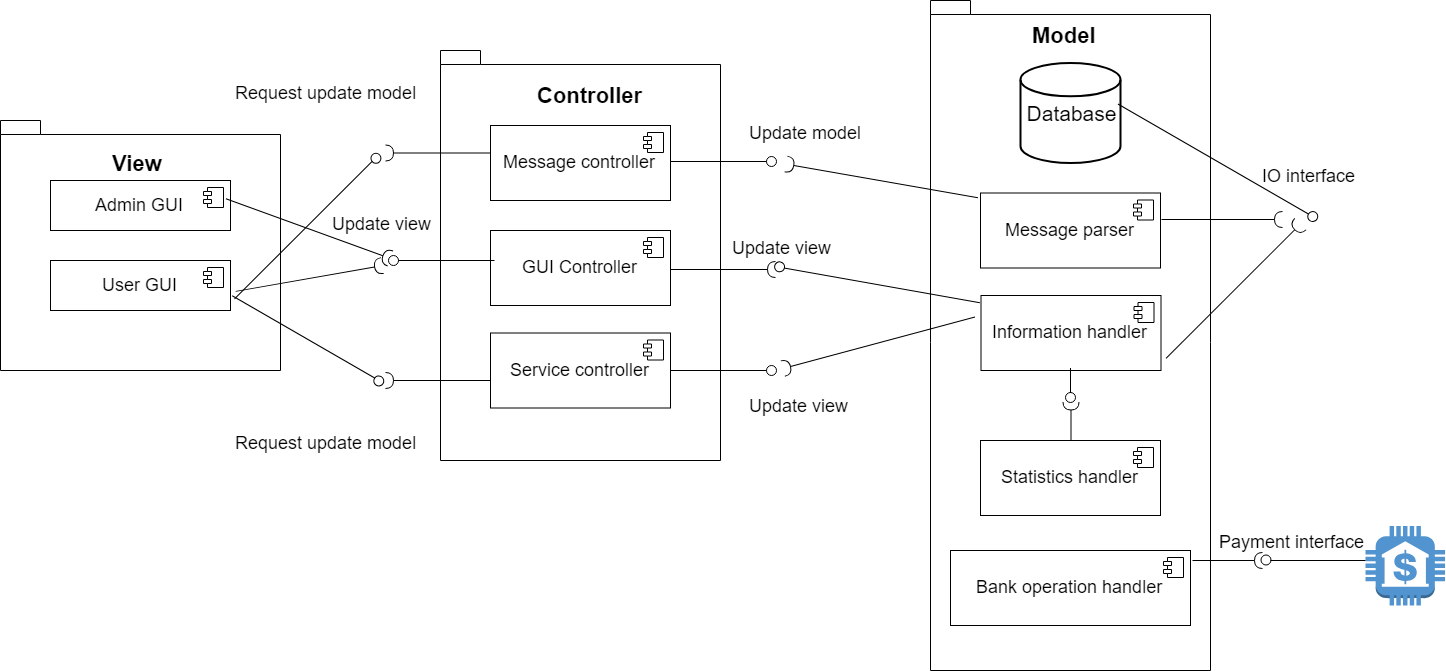
\includegraphics[width=1\textwidth]{KomponentuDiagrama.png}
    				\caption{Komponentų diagrama}
    				\label{fig:Komponentų diagrama}
			\end{figure}

	Sistema išskaidyta į 3 sluoksnius: View, Controller ir Model. View sluoksnyje talpiname vartotojo ir administratoriaus grafinius interfeisus, kurie bendrauja su Controller esančiais komponentais. Controller sluoksnyje esantys komponentai yra tarpiniai tarp grafinio interfeiso ir back-end. Komponentai, esantys jame, gavę grafinio interfeiso signalus juos apdoroja ir kreipiasi į Model, kuriame esantys komponentai pagrinde skirti duomenų bazės redagavimui. Norint atvaizduoti atnaujintą informaciją vartotojui, Model esantys komponentai perduoda informaciją į Controller ir pastarasis perduoda informaciją View, kur ją išvysta vartotojas.
	\pagebreak
	\subsection{Išdėstymo diagrama}
			\begin{figure}[h]
    				\centering
    				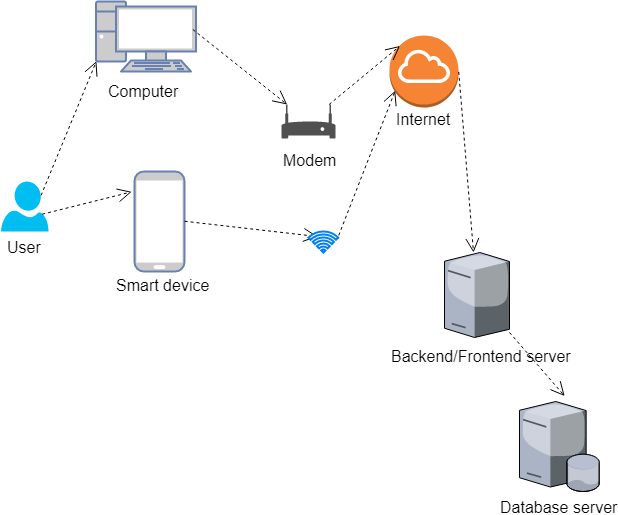
\includegraphics[width=0.75\textwidth]{Deployment.png}
    				\caption{Išdėstymo diagrama}
			\end{figure}

\section{Sistemos realizacija}
	\subsection{Duomenų bazės schema}
			\begin{figure}[h]
    				\centering
    				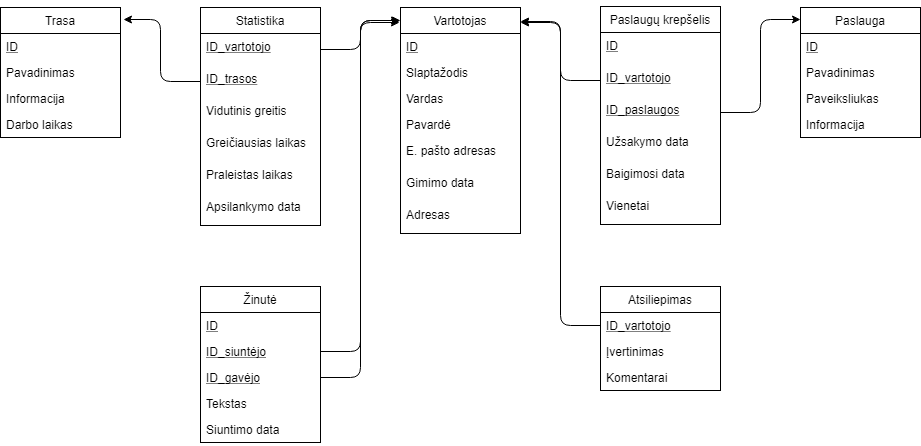
\includegraphics[width=1\textwidth]{Database_2.png}
    				\caption{Duomenų E-R modelis}
			\end{figure}
			
			\begin{figure}[h]
    				\centering
    				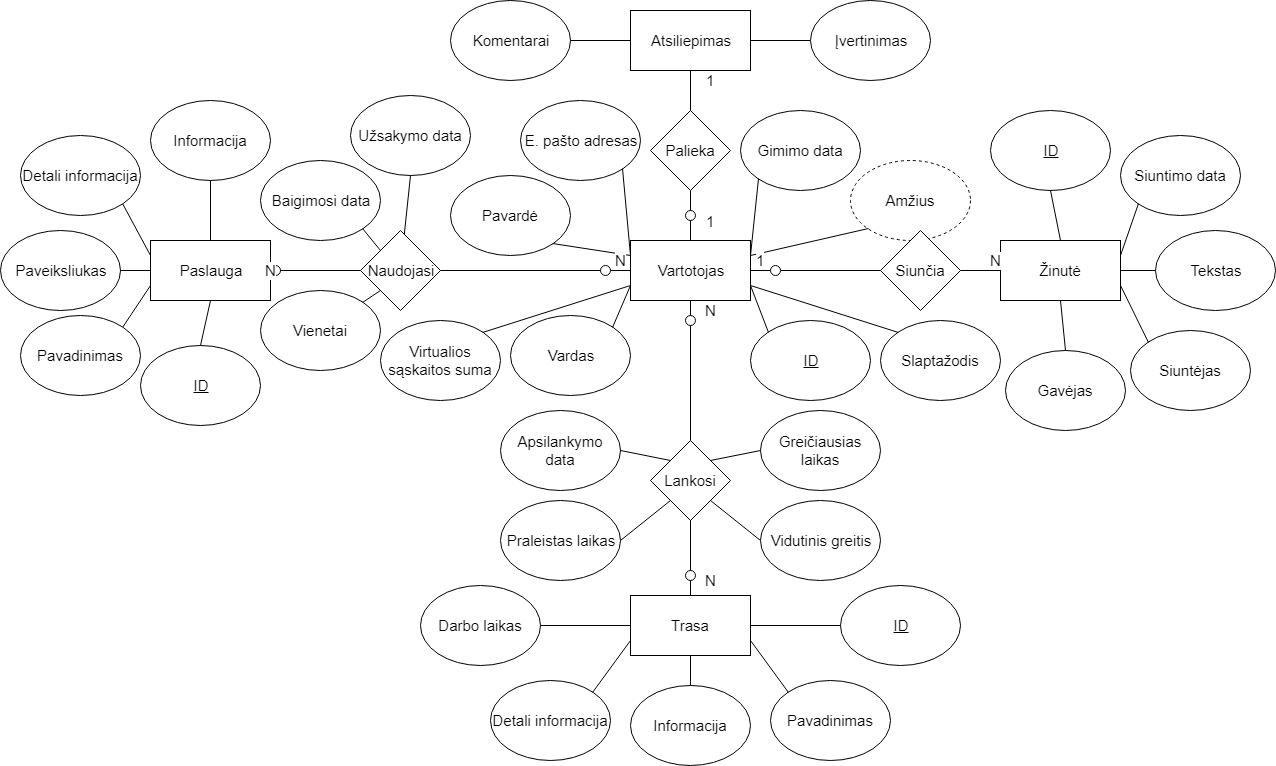
\includegraphics[width=1\textwidth]{Database2.png}
    				\caption{Duomenų bazės schema}
			\end{figure}
		

\section{Reikalavimų specifikacija}

\subsubsection{Pataisyta funkcinių reikalavimų specifikacija}
\begin{enumerate}
	\item Sistema seka vartotojų laiką, praleistą trasoje, pasinaudodama sekimo prietaisu.
	\item Sistema suteikia galimybę vartotojui įsidėti pinigų į virtualią piniginę.
	\begin{enumerate}
		\item Top-up metodu.
		\item Pervedimo būdu.
	\end{enumerate}
	\item Sekimo prietaisas fiksuoja greičiausią laiką, per kurį vartotojas įveikė trasą.
	\begin{enumerate}
		\item sistema saugo greičiausią laiką, per kurį vartotojas įveikė trasą.
	\end{enumerate}
	\item Vartotojo trasų laikai rodomi internetinėje aplikacijoje.
	\item Sistema internetinės aplikacijos pagalba vartotojui suteikia galimybę peržiūrėti orus.
	\begin{enumerate}
		\item Sistema turi pateikti dabartines oro sąlygas.
		\item Sistema turi pateikti ateinančių dienų orų prognozę.
		\begin{enumerate}
			\item temperaturą.
			\item drėgmę.
			\item kritulius.
			\item vėjo greitį.
		\end{enumerate}
	\end{enumerate}
	\item Internetinėje aplikacijoje vartotojas gali rašyti žinutes kitiems kurorto svečiams, administracijai ir maisto į kambarį tarnybai.
	\item Sistema vartotojui suteikia galimybę rašyti atsiliepimą apie jo viešnagę kurorte ir skirti viešą vertinimą kurortui.
	\item Internetinė aplikacija suteikia vartotojui galimybę peržvlegti statistiką.
	\begin{enumerate}
		\item Vartotojas turi galėti peržiūrėti savo statistiką.
		\item Vartotojas turi galėti peržiūrėti kurorto statistiką, jeigu ji patvirtinta administratoriaus.
		\begin{enumerate}
			\item Administratorius turi galėti patvirtinti arba atmesti naują statistiką apie kurortą.
		\end{enumerate}
	\end{enumerate}
	\item Sistema vartotojui suteikia galimybę peržiūrėti paslaugų kainas, tiekėjų sąrašą ir kiekvienos įrangos technines charakteristikas.
	\item Sistema per aplikaciją vartotojui suteikia galimybę užsisakyti paslaugas.
	\begin{enumerate}
		\item Užsisakyti maisto į viešbučio kambarį.
		\item Rezervuoti slidinėjimo įrangą.
	\end{enumerate}
	\item Vartotojas turi galimybę užrezervuoti slidinėjimo trasą nurodant: trasos pavadinimą, telefono numerį, slidinėtojų skaičių ir rezervacijos laikotarpį.
	\item Vartotojas gali matyti informaciją apie slidinėjimo trasą: pavadinimą, sunkumą, rūšį, nuomos kainą, užimtumą.
	\item \textit{Sistema vartotojui suteikia galimybę peržiūrėti jo užsakytas paslaugas}
	\item Sistema suteikia galimybę keisti vertinimą.
	\item Sistema suteikia galimybę pasirinkti laikotarpį, kuriuo filtruoti lankytas trasas.
	
\end{enumerate}


\subsubsection{Pataisyta nefunkcinių reikalavimų specifikacija}
\begin{enumerate}

	
	\item Sistema neleidžia vertinti kurorto kelis kartus tam pačiam asmeniui dažniau nei kartą per 2 mėnesius.
	\item Sistema leidžia vartotojui už paslaugas atsiskaityti e-bankininkyste.
	\item Slidinėjimo trasų įrangos bei kambarių pavadinimams maksimaliai skiriama 64 simboliai.
	\item Slidinėjimo trasos ilgis vaizduojamas vieno skaičiaus po kablelio tikslumu
	\begin{enumerate}
		\item Ilgio matavimo vienetas - kilometras
	\end{enumerate}
	\item Slidinėjimo trasos statumas vaizduojamas vieno skaičio po kablelio tikslumu
	\begin{enumerate}
		\item Statumo matavimo vienetas - procentai
	\end{enumerate}
	\item Slidinėjimo trasų, įrangos bei apgyvendinimo įstaigos laisvų vietų skaičius rodomas vienetų tikslumu.
	\item Slidinėjimo trasų, įrangos bei apgyvendinimo įstaigos kainos pateikiamos centų po kablelio tikslumu (10,11eu)
	\item Data turi būti vaizduojama formatu YYYY-MM-DD
	\begin{enumerate}
		\item YYYY - metai
		\item MM - mėnuo
		\item DD - diena
	\end{enumerate}
	\item Laikas turi būti vaizduojamas formatu hh:mm 24 valandų formatu (21:47)
	\begin{enumerate}
		\item hh - valandos 24 valandų formatu
		\item mm - minutės
	\end{enumerate}
	\item Svečių skaičiui rezervacijos formoje maksimaliai skiriama 3 skaičiai
	\item Orų temperatūra rodoma vienetų tikslumu. Matavimo vienetas - celsijus
	\item Įrangos dydžiai - europietiški. Vaizduojama vienetų tikslumu
	\item Keičiant naršyklės dydį, tinklapio vaizdas pritaikomas automatiškai(Responsive design).
	\item Sistema turi veikti 95proc laiko per dieną. Tai yra leidžiama neveikti 1 valandą 10 min.	
	\item Vartotojui rezervuojant paslaugas sistema turi patikrinti, ar duomenys įvesti korektiškai
	\item Vartotojui rezervuojant paslaugas sistema rezervacijai turi priskirti unikalų numerį.
	\item Modifikuojama tinklapio atsarginė kopija po kiekvieno informacijos atnaujinimo apie slidinėjimo kurortą, orų prognozes, slidinėjimo trasas, įrangą, apgyvendinimo įstaigą, jų užimtumą bei po kiekvienos esybės registracijos ir įvestos informacijos pakeitimo.
	\item Sistemoje turi būti įdiegtos apsaugos priemonės nuo duomenų sugadinimo, praradimo, klaidingų duomenų įvedimo į duomenų bazėje.
	\item Po kiekvienos sėkmingos operacijos pakeitimai turi būti išsaugoti duomenų bazėje.
	\item Nepavykus prisijungti arba negavus duomenų iš duomenų bazės, sistema turi informuoti vartotoją, parodydamas klaidos pranešimą
	\item Didžiausia leistina tinklalapio apkrova yra 10000 vartotojų vienu metu
	\item Tinklalapio didžiausias leistinas reakcijos laikas, neįvertinant interneto greičio, turi būti ne didesnis kaip 2 sekundės.
	\item Užklausos vykdymo laikas turi būti ne didesnis nei 3 sekundės
	\item Konkrečios slidinėjimo trasos, įrangos, kambario, jų užimtumo paieškai duomenų bazėje turi būti sugaišta ne ilgiau nei 3 sekundės
	\item Tinklapis pasiekiamas prisijungiant iš bet kurio IP adreso
	\item Pradinėje sistemoje turi būti administratoriaus prisijungimo duomenys
	\item Pasirinkimų lentelė turi turėti bent 5 pradines užpildytas eilutes su informacija apie slidinėjimo trasas, įrangą, kambarius. Šią informaciją įveda įgaliotas įmonės administratorius interfeisu.
	\item Sistemos turi funkcionuoti lietuvių ir anglų kalbomis
	\item Įmonės darbuotojai turi būti apmokomi naudotis sistema
	\item Pakeitimai turi būti įvykdyti ne vėliau nei per 7 darbo dienas po sėkmingo testavimo.
	\item Visi vartotojo atliekami veiksmai turi būti saugomi laikinoje duomenų bazėje, kad atradus klaidą tinklalapyje būtų galima testavimo metu atkurti konkrečia klaidą
	\item Pastebėtos ar esybės praneštos klaidos turi būti ištaisytos kaip galima greičiau.
	\item Į vartotojo atsiųstus laiškus su pastebėjimai ir skundais reikia atsakyti automatine žinute.
	\item Sistema atnaujinti reikia tuo metu, kai yra mažiausias vartotojų srautas
	\item Internetinė aplikacija turi veikti bet kuriame įrenginyje, kuris turi naršyklę, palaikančią HTML5 standartą.
	\item Visi duomenys apie sistemą saugomi duomenų bazėje, o prie jos prieigą turi tik įgalioti asmenys.
	\item Atsarginė duomenų bazės kopija turi būti daroma reguliariai kas 7 darbo dienas.
	\item Jeigu esybė neaktyvi ilgiau nei 15 minučių, vartotojas automatiškai atjungiamas.
	\item Kuriant sistemą projekto komandai draudžiama naudotis nelegalia programine įranga
	\item Duomenų perdavimas ir saugojimas neturi pažeisti LR asmens duomenų teisinės apsaugos įstatymo.
	\item Esybių asmeniniai duomenys turi būti įslaptinti t.y. tinklapyje negali būti saugomi nekoduoti duomenys
	\item Minimali sąskaitos papildymo suma yra 3€

\end{enumerate}

\section{Žodynas}
\begin{enumerate}
	\item Internetinė aplikacija - Mūsų kuriama android programėlė
	\item Administratorius - Sistemą prižiūrintis žmogus
	\item Vartotojas - Slidinėjimo kurorto klientas, naudojantis programėlę
	\item Susirašinėjimas - Dviejų vartotojų žinučių grandinė
	\item Virtuali piniginė - Piniginė, kurioje esančiais pinigais galima atsiskaityti už pramogas
	\item Sekimo prietaisas - Įrenginys, siunčiantis savo poziciją sistemai
	\item Atsiskaitymų sistema - Sistema, kuri apdoroja bankinius pinigų pervedimus
	\item Duomenų bazė - Organizuota duomenų struktūra
	\item Vartotojo statistika - Duomenys, renkami apie vartotoją
	\item Sutartys - Rašytinis susitarimas tarp vartotojo ir slidinėjimo kurorto
	\item Kurorto statistika - Duomenys renkami apie kurortą
	\item DAO - Data Access Object
\end{enumerate}

\end{document}